\documentclass[11pt,a4paper]{report} % TODO maybe use 'report' instead, this way I could use \chapter
\usepackage[utf8]{inputenc}
\usepackage[english]{babel}
\usepackage[T1]{fontenc}
\usepackage{amsmath}
\usepackage{amsfonts}
\usepackage{amssymb}
\usepackage{graphicx}
% \usepackage{subcaption}%subfigures, not compatible with the 'caption' package
\usepackage[breaklinks=true,hidelinks]{hyperref}
% \usepackage[breaklinks=true]{hyperref}
% \usepackage[xindy, toc, nonumberlist]{glossaries}
\usepackage[toc, acronym, nonumberlist]{glossaries}
% \gls{label} to invoke the entry.
% \glsreset{label} to reset the first occurence of the entry.
% \acrlong{label} to print the long version of the acronym.
% \acrshort{label} to print the short version of the acronym.

\usepackage{todonotes}

\usepackage{etoolbox}
\AtBeginEnvironment{quote}{\itshape} 	% https://tex.stackexchange.com/questions/235852/how-to-make-all-quotes-italicised
										% 

\usepackage{textcomp} % For \textmu, among other things.
\linespread{1.1}


% %%%%%%%%% vvvvvvv
% % Anthony Debruyn 
% \let\oldCaption\caption
% \renewcommand{\caption}[2]{
% \oldCaption[#1]{{\small\bfseries #1: }\small #2}
% }
% %%%%%%%%%%%%%%%%%%%%%%%%%%%%%%%%%%%%%%%%%%%%%%%%%%%%%%%
% % NEW STYLES
% %%%%%%%%%%%%%%%%%%%%%%%%%%%%%%%%%%%%%%%%%%%%%%%%%%%%%%%
% \captiondelim{ -- }
% \captionnamefont{\small\bfseries}
% \captiontitlefont{\small}
% \precaption{\rule{\linewidth}{0.4pt}\\}
% % Anthony Debruyn
% %%%%%%%%% ^^^^^^^



\usepackage{geometry}
\geometry{
  top=0.8in,
  inner=0.7in,
  outer=0.7in,
  bottom=1in,
  headheight=3ex,
  headsep=5ex,
}

% \usepackage{palatino}
\usepackage{tgtermes}
% \renewcommand{\familydefault}{\sfdefault}

\usepackage{fancyhdr}

\usepackage[margin=1cm, small]{caption}



\usepackage{mdframed}
\newmdenv[
  topline=false,
  bottomline=false,
  rightline=false,
  skipabove=0,%Space above the frame. I want none so that it's close to the def title.
  skipbelow=2em,%Below the frame. Leave it some room to breath.
  innerbottommargin=0,%Margin between the bottom of the text and the bottom of the frame.
  innertopmargin=0,%Margin between the top of the text and the top of the frame.
]{siderules}

% \usepackage[]{natbib}
\usepackage[numbers]{natbib}
\usepackage{amsthm}%theorems
\newtheoremstyle{customdef}%
	{\topsep}% above the theorem
	{\topsep}% below the theorem
	% {\itshape}% body
	{}% body
	{0pt}% indent
	{\bfseries}% head
	{}% punctuation between head and body
	{ }% Space after theorem head
	{\thmname{#1}\thmnumber{ #2}: \thmnote{#3}}
\theoremstyle{customdef}
\newtheorem{definition}{Definition}

% Arg1: Title of the definition
% Arg2: Label
\newenvironment{defi}[2]
 {\begin{definition}[#1]\label{#2}\end{definition}\begin{siderules}}
 {\end{siderules}}
 % {\begin{definition}[#1]\label{#2}\end{definition}\vspace{-1em}\begin{siderules}\vspace{-0.5em}}
 % {\vspace{-0.5em}\end{siderules}}


%https://tex.stackexchange.com/questions/84478/how-to-format-title-and-abstract
\renewenvironment{abstract}{%
\begin{center}\begin{minipage}{0.85\textwidth}
\rule{\textwidth}{1pt}}
{\par\noindent\rule{\textwidth}{1pt}\end{minipage}\end{center}}


\makeglossaries
\newglossaryentry{gl:netlist}
{
	name=netlist,
	description={File descripting the connectivity of an architecture.
				Such a list can either be \textit{pin-oriented} or \textit{net-oriented}.
				The former focuses on the design components or their associated nets, the later on the nets and their associated components.
				\newline
				A netlist can either be hierarchical or flat.}
}

\newglossaryentry{gl:primitive}
{
	name=primitive,
	description={In a netlist, a primitive is a definition which does not include any instance.
				As such, a flat netlist only contains primitives}
}

\newacronym{ac:rtl}{RTL}{Register Transfer Level}

\newglossaryentry{gl:rtl}
{
	name=register transfer level,
	description={Level at which are described the signals and the values they should take}
}

\newacronym{sa}{SA}{Simulated Annealing}
\newacronym{ts}{TS}{Tabu Search}


\usepackage{titling}
\setlength{\droptitle}{10em}

\author{Quentin Delhaye}
\date{September 2017}
\title{Automated System Partitioning for Efficient 3D Circuit Integration \\ \vspace{.5em} \hrule \vspace{.5em} \large Reaserch Progress Report}

\begin{document}
% TODO When several references are cited at the same time, sort them alphabetically so that they appear in order in the pdf.

\pagenumbering{gobble}% Remove page numbers (and reset to 1)

% \maketitle

% \vspace{5cm}


% ##########  ########   ##########  ##         #########  
%     ##         ##          ##      ##         ##         
%     ##         ##          ##      ##         ##         
%     ##         ##          ##      ##         ######     
%     ##         ##          ##      ##         ##         
%     ##         ##          ##      ##         ##         
%     ##      ########       ##      #########  #########  

\newgeometry{
  top=0.3in,
  inner=0.7in,
  outer=0.7in,
  bottom=1in,
  headheight=3ex,
  headsep=5ex,
}
\begin{titlepage}
\begin{center}

\includegraphics[width=7cm]{img/logo-polytech-ULB-FR.jpg}

\includegraphics[width=5cm]{img/beams}
\end{center}
~\vspace{5cm}
\begin{center}
 {\LARGE Automated System Partitioning for Efficient 3D Circuit Integration \\ \vspace{.5em} \hrule \vspace{.5em} \Large Research Progress Report\\}
 % ----------------------------------------------------------------
 \vspace{1.5cm}
 {\large Quentin \textsc{Delhaye} -- September 2017}\\[5pt]
 \vspace{3.5cm}

\begin{abstract}
Who does not want a more powerful and compact chip to process their funny cat videos?
The industry has been fulfilling this wish for decades, but struggles to keep it financially viable.
It is becoming obvious that the classic 2D architectures are being limited by their own technology.
We need to go beyond the 2D paradigms and explore the third dimension.
Numerous research groups are working on different aspects of this vast and problem-prone subject.

We are currently working on automating the partitioning of 2D architectures that is still mostly done by hand.
To do so, we are developing a solution interfacing with popular production sofwtares and standards that will process the placed and routed 2D design, extract the underlying hypergraph and statistics, cluster it, partition it and re-generate netlists for each die.

As of now, we have a hypergraph and statistics extractor as well as a naive clustering solution for bipartitioning any architecture.
Although existing partitioning libraries were used, new weights metrics have been studied.
The impact of clustering granularity on inter- and intra-cluster connectivity has also been under our scope.

Some intermediate results showed a gain of up to 77\% in total wire length on some architectures when going 3D, and clusters containing 1000 to 5000 gates appears to be the sweet spot in terms of inter-cluster nets versus inter-cluster wire length.

% Who does not want a more powerful and compact chip to process their kinky videos?
% The industry has been fulfilling this wish for decades, but struggles to keep it financialy viable.
% It is becoming obvious that the classic 2D architectures are being limited by their own technology.
% As a famous space ranger once said: “To infinity... and beyond 2D!”
% We need to go beyond the 2D paradigms and explore the third dimension.
% Numerous research groups are working on different aspects of this vast and problem-prone subject.

% We are currently working on automatizing the paritioning of 2D architectures that are still mostly done by hand.
% To do so, we are developing a solution interfacing with popular production sofwtare and standards that will process the placed and routed 2D design, extract the underlying hypergraph and statistics, cluster it, partition it and re-generate netlists for each die.

% As of now, we have a hypergraph and statistics extractor as well as a naive clustering solution for bipartitioning any architecture.
% Although existing partitioning libraries were used, new weights metrics have been studied.
% The impact of clustering granularity on inter- and intra-cluster connecticity has also been under our scope.

% In the near future, the generation of partitioned netlists and multiple dies partitioning will be addressed.
\end{abstract}
 \vfill
\end{center}
\end{titlepage}







\clearpage

% Change the geometry after the title page to shrink the margins a bit.
\newgeometry{
  top=1in,
  inner=1.5in,
  outer=1in,
  bottom=1in,
  headheight=3ex,
  headsep=5ex,
}

% If we do this before changing the geometry, the header is fucked up.
\pagestyle{fancy}
\fancyhf{}
\chead{Automated System Partitioning for Efficient 3D Circuit Integration}
\cfoot{\thepage}

\thispagestyle{empty}

\tableofcontents

\clearpage

\thispagestyle{empty}

\pagenumbering{roman}

% \glsaddall
\printglossaries

\clearpage

\thispagestyle{plain} % Basic style, only the page number, but only for this page. I don't want the fancy header above the introducing quote.

\begin{quote}
Imagine you are the heir to an antic civil contractors family.
Since the dawn of time, your family has managed their terrain as a parking lot.
First it was for horse-drawn caravans, bulky and rare.
Along the years, the vehicles became less ponderous and cheaper, thus more common.
Nowadays, they are as small as they can get and ever cheaper.
What are now called “cars” fill your terrain and more are piling up at the entrance.
You need them on your domain if you want to prosper.
Will you still wait for more clever engineers to develop smaller cars, or will you finally build a new floor and go 3D?


% Imagine you are an antic civil contractor asked to handle high density parking for horse-drawn caravans.
% You have a fixed area terrain on which you can fit so much cars.
% Along the years, they become smaller and less bulkier, but that scaling tend to slow down and you still need to fit more and more of them on your parking.
% You now have to make a choice: Do you spend time and money to engineer expensive cars using new materials, or do you finally add a second floor to your parking?
\end{quote}





% ########   ##      ##  ##########  ########     #####    
%    ##      ###     ##      ##      ##     ##  ##     ##  
%    ##      ## ##   ##      ##      ##     ##  ##     ##  
%    ##      ##  ##  ##      ##      ########   ##     ##  
%    ##      ##   ## ##      ##      ##   ##    ##     ##  
%    ##      ##     ###      ##      ##    ##   ##     ##  
% ########   ##      ##      ##      ##     ##    #####    

\chapter{Motivation: Why do we want to go 3D?}
\pagenumbering{arabic}% Arabic page numbers (and reset to 1)

Stability, security, performance, we always want more.
The same goes for \glspl{ic}.
They are everywhere: in your dishwasher, your phone, your car, your heating system, maybe even inside your body.

Take the figure~\ref{fig:trans}.
This little piece of technology is making the world go round.
But the world is greedy, it always wants more.
For a very long time, more meant smaller transistors, but in the recent years, this scaling faced ever complex challenges.

\begin{figure}[!h]
\centering
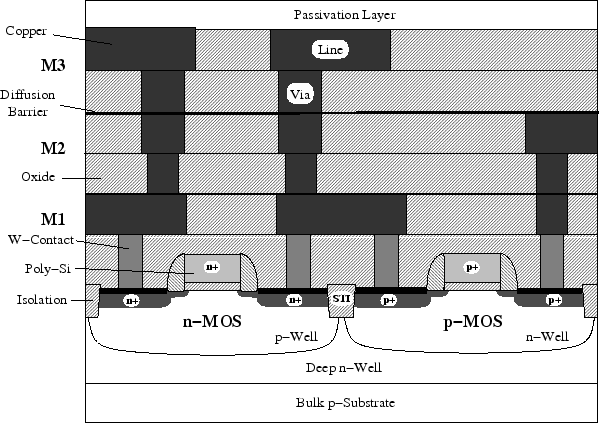
\includegraphics[width=.8\textwidth]{img/trans.png}
\caption{Schematic section view of an IC (\citet{Wittmann2007}).
From bottom to top, we have: the substrate and the active layer with the transistors, \textit{i.e.} \gls{feol}; the metal layers (M1, M2, M3), \textit{i.e.} the \gls{beol}.}
\label{fig:trans}
\end{figure}

% http://www.eetimes.com/author.asp?doc_id=1321536
% https://www.economist.com/news/science-and-technology/21652051-even-after-moores-law-ends-chip-costs-could-still-halve-every-few-years-beyond
Beyond the 28nm technology node, the cost per transistor has increased for the first time (figure~\ref{fig:cost-trans}).
Not only are the transistors more expensive to manufacture, but the thinner wires also implies more intricate \gls{beol} layers patterning, further increasing the cost.
Since then, it kept on getting more expensive and less cost effective.
Yes, the industry still manages to cram more and more transistors on the same surface of silicon, but its profitability is stagnating if not crumbling.

\begin{figure}[!h]
\centering
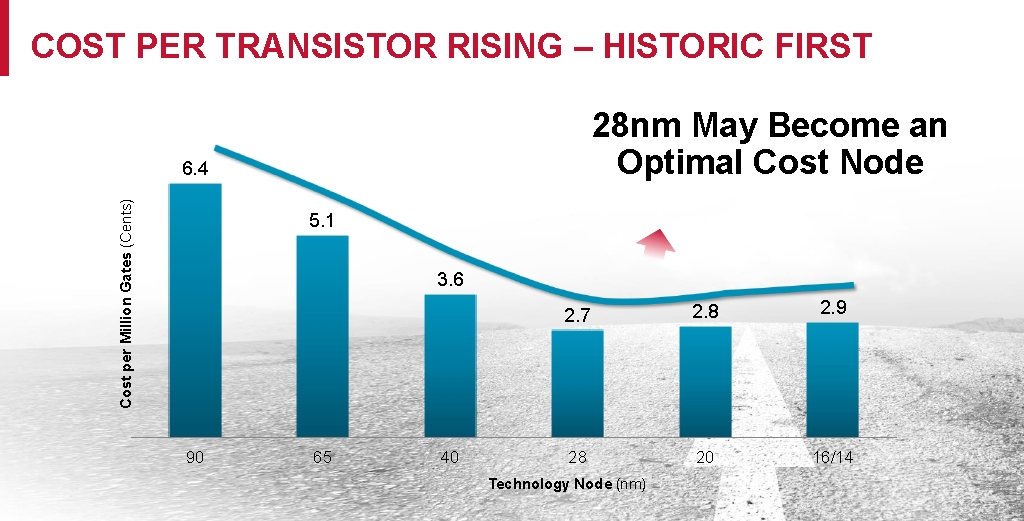
\includegraphics[width=.8\textwidth]{img/cost-trans.jpg}
\caption{Cost of transistors per technology node (\citep{electroiq2014}).}
\label{fig:cost-trans}
\end{figure}

But money is not the only limitation in this situation.
Even assuming the technology can keep up with the scaling, and the \gls{itrs} expects the 5nm node by 2020, another problem arises.
With the shrinking of transistors, the gate delay decreases, but the wire delay increases (see figure~\ref{fig:delay}).
The wire delay is already dominant since the 180nm node in 1999, but beyond 16nm, it is ten thousandfold more.

\begin{figure}[!h]
\centering
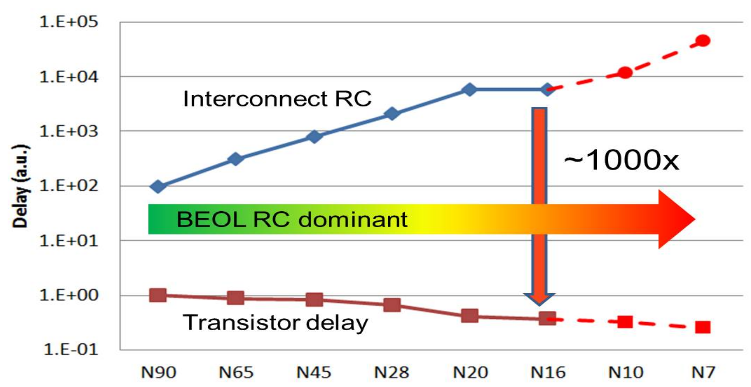
\includegraphics[width=.8\textwidth]{img/beol-delay.png}
\caption{Interconnect RC (wire) delay versus Transistor (gate) delay (\citep{Yeap2013}).}
\label{fig:delay}
\end{figure}

To circumvent this increasing delay, engineers need to insert repeaters and buffers in the design, which occupy precious space on the die.
The \gls{itrs} is aware of this situation.
That is why in 2014, its committee reorganized the working groups into seven focus topics.
Some of them, such as “System Integration” and “Heterogeneous Integration”, have for mission to explore and develop 3D integration technologies, \textit{i.e.} stacking several layers of transistors, effectively increasing the number of cells per unit area.

\begin{figure}[!h]
\centering
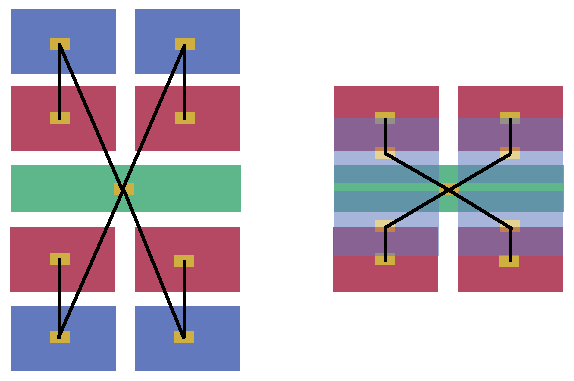
\includegraphics[width=.4\textwidth]{img/2dto3d.png}
\caption{Transformation from a 2D to a 3D architecture. As the dies are stacked, the farthest blocks are brought closer and the interconnections are shortened.}
\label{fig:2dto3d}
\end{figure}

3D ICs can help save the day by reducing the area, improving the yield and casting aside the need for repeaters and buffers; once the dies are stacked and the length reduced, there won't be any need for them.
Indeed, as logical block are stacked and brought closer to each other, their interconnection is shorter (see figure~\ref{fig:2dto3d}).
The aim of system partitioning is to shorten the longest nets and preserve the shortest.

However, 3D is not around the corner just yet.
Amongst other challenges, the industry still lacks proven toolchains capable of designing those 3D ICs.
This is where we intervene: by intending to develop a complete toolchain automating the design and partitioning of 3D ICs.\\

In this report, we will see what is the scope of this subject (chapter~\ref{chap:soa}), present some of the challenges 3D ICs face (chapter~\ref{chap:challenges}), explain what we developed to contribute to the research effort (chapter~\ref{chap:work}), discuss some preliminary results (chapter~\ref{chap:results}) and take a peek behind the door of the future of this project (chapter~\ref{chap:future}).


% \section{Why is 2D not enough anymore?}
% \begin{itemize}
% 	\item MONEY
% 	\item Gate capacitance increasing
% 	\item Manufacturing. 
% \end{itemize}

% \todo[inline]{Moore and Rock Laws => “more than Moore technologies”}
% Cost effectiveness scaling, loss of rentability after 28nm
% + see feedback 2016-08-31


% Problems with 2D:
% \begin{itemize}
% 	\item CMOS scaling and photolitography limitations
% 	\item Leakage current: thinner gate leads to sub-threshold leakage
% 	\item Wire delay
% \end{itemize}

% Advantages of 3D:
% \begin{itemize}
% 	\item Reduce the interconnect delay
% 	\item Increase the density (number of transistors per unit area)
% 	\item Heterogeneous technology integration. We can use an $N+1$ technology node fo the critical units and fall back to $N$ or even $N-1$ for the others.
% 	This way, we can reduce the cost of the chip without impeding its performance.
% 	\item Heterogeneous modules integration.
% 	A single chip does not need to be memory or logic only.
% 	Using a clever 3D integration, each die layer could be either logic, memory, sensors, etc.
% \end{itemize}




%  #######     #####       ###     
% ##     ##  ##     ##    ## ##    
% ##         ##     ##   ##   ##   
%  #######   ##     ##  ##     ##  
%        ##  ##     ##  #########  
% ##     ##  ##     ##  ##     ##  
%  #######     #####    ##     ## 

% Definitions inspired from Selvakkumaran2006 (Karypis was a co-author)
\chapter{State of the Art: How do we go 3D?}\label{chap:soa}

In this chapter, we will first define the basic terms (section~\ref{sec:def}) needed to discuss partitioning (section~\ref{sec:part-algo}).
Said discussion will focus on some of the most popular partitioning algorithms, their implementation and why hypergraphs are used.
In chapter~\ref{chap:work}, we will present \texttt{PHONEY}, our software implementing those methods.

Next, we will present some physical integration techniques (section~\ref{sec:int-flav}) and existing design flows (section~\ref{sec:flows}).






\section{Definitions}\label{sec:def}
The following section will define the basic terms and concepts used in this work.

% TODO For some reason, the first letter of some definitions is not printed. That's why it's repeated.
\begin{defi}{Hypergraph}{def:hypergraph}
A \emph{hypergraph} $H = (V, E)$ is a set of vertices $V$ and a set of hyperedges $E$.
Each hyperedge is a subset of vertices and its size is the cardinality of this subset.
Each vertex $v$ and hyperedge $e$ is associated with a weight $w(v)$ and $w(e)$, respectively.
\end{defi}

\begin{figure}[!h]
\centering
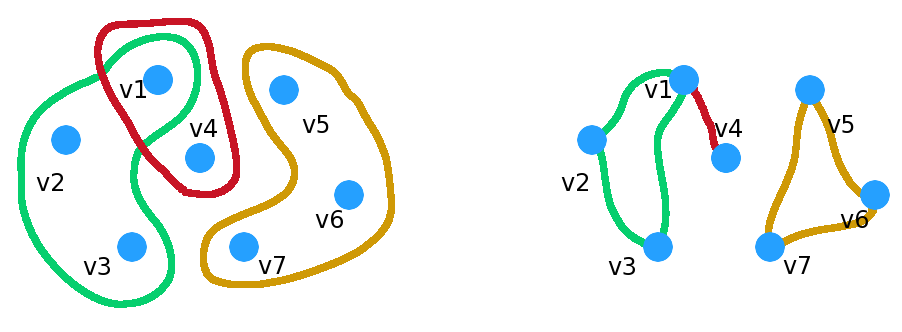
\includegraphics[width=.9\textwidth]{img/hypergraph-graph.png}
\caption{On the left, a hypergraph and on the right, the corresponding graph.}
\label{fig:hypergraph-graph}
\end{figure}

\begin{defi}{k-way partitioning}{def:k-way-part}
A \emph{k-way partitioning} is a decomposition of $V$ into $k$ disjoint subsets $V_1, V_2, ... , V_k$, such that $\bigcup_i V_i = V$.
Each of these $k$ subsets is called a partition.

When $k = 2$, the decomposition is called a bipartitioning.
\end{defi}

\begin{defi}{Cutsize}{def:cutsize}
The \textit{cutsize} of a k-way partitioning is the sum of the weights of the hyperedges spanning several partitions, \textit{i.e.} hyperedges containing vertices from different partitions.
\end{defi}

\begin{defi}{Balanced partitioning}
A A partitioning is balanced with respect to a constraint $[l, u]$, with $l < u$, when for each partition $V_i$, $l \leq \sum_{v \in V_i} w(v) \leq u$.
\end{defi}

\begin{defi}{Balanced partitioning problem}
GGiven a hypergraph $G$ and a balancing constraint $[l, u]$, the balanced partitioning problem is to compute a $k$-way partitioning with the minimal cutsize and respecting the balancing constraint.
\end{defi}

% \subsubsection{Complexity}

% \begin{defi}{Non-deterministic Turing Machine}{def:nd-tm}
% In this kind of Turing machines, the transition \emph{rule} becomes a transition \emph{function}.
% It means that at a given state, with a given symbol, it has many possible execution instead of just the one with a deterministic Turing machine.
% We can see that as the machine always taking the best possible guess, leading to a finishing state in the end, or the machine is branching into all the possible states from the point of decision.
% \end{defi}


% \begin{defi}{NP}{def:np}
% Acronym for ``non-deterministic polynomial-time".
% A ``yes"-instance can be found in polynomial-time by a non-deterministic Turing machine, and this solution can be verified in polynomial-time by a deterministic Turing machine.
% \end{defi}

% \begin{defi}{NP-hard}{def:np-hard}
% Acronym for ``non-deterministic polynomial-time hard".
% ~\newline{}\noindent Note: it has never been proven that there is no polynomial-time algorithm to solve those problems.
% Informally, it means that those problems are at least as hard as the hardest problems in NP.

% The problem size grows linearly, but the time needed to solve it grows faster than any polynomial function.
% \end{defi}

% \begin{defi}{NP Complete}{def:np-comp}
% A problem is NP complete when it is both NP and NP hard at the same time.
% Although the solution can be verified in polynomial time, there is no known algorithm to find this solution quickly.
% The problem to know if such algorithm exist is the “P $=$ NP” problem.

% An NP-complete problem differs from a regular NP problem in the sense that a problem is NP-complete if every other problem in NP can be reduced to it.ea
% \end{defi}

% \begin{defi}{P=NP}{def:p-np}
% Problem asking if there exist polynomial time algorithm solving NP-complete problems (an by corollary all NP problems).
% \end{defi}




\section{The Usual Suspects -- Partitioning algorithms}\label{sec:part-algo}
As the problem of graph partitioning is NP-complete~\citep{Garey1976}, it needs heuristics to be solved.
% The first solutions developed focused on being efficient even if suboptimal.
Typical algorithms include local search based solutions (such as \glsfirst{kl}~\citep{Kernighan1970} and \glsfirst{fm}~\citep{Fiduccia1982}), simulated annealing~\citep{Johnson1989}, %genetic algorithm \citep{Bui1996} \citep{Maini1996} \citep{Kim2011} \citep{Shanavas2014}, 
tabu search \citep{Pirlot1996}, etc.
To scale up with the problem size and handle millions of nodes, the multilevel paradigm was developed.
% A lot of solutions have been developed along the years to solve various partitioning-related problems (\citep{Tsourakakis2014}, \citep{export:183714}).
Nowadays, as we reach graphs with billions of nodes, new methods need to be researched (\citep{Tsourakakis2014, export:183714}).

In this section, we present some of the most popular partitioning methods.






\subsection{Kernighan-Lin Algorithm}
\gls{kl} is a partitioning method published by \citet{Kernighan1970}, based on gain cell swap.
The idea is to randomly bipartition an undirected graph and improve its cutsize by swapping pairs of nodes across the partition.

During each pass of the algorithm, we compute the cost of each cell in both partitions $P_p$, with $p \in \{1,2\}$:
\begin{itemize}
	\item External cost of cell $x$ belonging to partition $P_1$: \[E_x = \sum_{i \in P_2} c(x,i)\] with $c(x,i)$ the weight of the edge between the nodes $x$ and $i$.
	\item Internal cost of cell $x$ belonging to partition $P_1$: \[I_x = \sum_{i \in P_1} c(x,i)\]
\end{itemize}

From these two costs, we can compute the gain of swapping the cells $x$ and $y$:
\[gain(x,y) = (E_x - I_x) + (E_y - I_y) - 2 \cdot c(x,y)\]

At each step of the pass, we (i) compute the gain of all unlocked nodes, (ii) swap the pair with the highest gain and lock both nodes into their new partition, (iii) record the current cutsize.
When all pairs have been swapped and if the cutsize has not decreased, we stop. Otherwise, we unlock all the nodes and start a new pass using the $m$ first swaps leading to the minimal cutsize.\\

A limitation that may seem obvious is that the vertices need to have the same weight if we want the bipartition to be balanced.
There is however a workaround (\citet[p. 41]{KahngAndrewB.Lienig2011}). We first define a unit-cost weight $W_u$ that is the greatest common divisor of all node weights $W_n$.
Then, we instantiate all nodes $W_n/W_u$ times with a weight $W_u$ and link those instances together using infinite-weight edges.
Those edges will become high priority whenever a portion of the node has crossed the partition boundary, forcing \gls{kl} to keep the instances together.


\paragraph{Application to circuits}
In order to obtain an undirected weighted graph $G$ from the circuit, we can use the \gls{gl:kclique} model: Each net that contains $k$ gates becomes a $k$-clique in $G$.
In a $k$-clique, each node can have a weight of $\frac{1}{k-1}$, and if an edge already exists, its weight is simply summed instead of being duplicated.
% A further study on weights is discussed in section~\ref{sec:work}.


\paragraph{Time complexity}
We need $\mathcal{O}(n^2)$ to update the gain of $n$ nodes, and $\mathcal{O}(n^3)$ to compare the $\mathcal{O}(n^2)$ pairs and choose the maximum gain.
This leads to a $\mathcal{O}(n^3)$ time complexity.
However, if the nodes are sorted and the comparison cleverly ordered, it can drop to $\mathcal{O}(n^2\log{}n)$~\citep*{Cormen2009, Dutt1993}.







\subsection{Fiduccia-Mattheyses Algorithm}
\gls{fm} is a method to bipartition hypergraphs, developed by~\citet{Fiduccia1982}.
In contrast with \gls{kl}, \gls{fm} is based on cell moves instead of cell swaps.
There is then no need to compute lots of gains, but a balance constraint becomes necessary to ensure that a cell move does not disbalance the bipartition.

Like for \gls{kl}, the first bipartition is random and will be improved upon successive passes.
At the beginning of the first pass, we compute the gain of each cell $x$: \[gain(x) = FS(x) - TE(x)\]
with $FS(x)$ the number of nets having $x$ as its only cell in $P_1$ and $TE(x)$ the number of nets containing $x$ and being entirely located in $P_1$.

At each step of the pass, we (i) choose a free cell with maximum gain which move is allowed by the balance constraint, (ii) move it and lock it, (iii) update the gain of the impacted cells and (iv) record the current cutsize.

When the cutsize is not improved at the end of a pass, we stop. Otherwise, we keep the fist $m$ moves that led to the minimum cutsize and begin a new pass.


\paragraph{Application to circuits}
As \gls{fm} already works on hypergraphs, the application to circuits is fairly immediate: Each net becomes an hyperedge and each cell becomes a vertex.

\paragraph{Time complexity}
Since we only need to update the gain of cell movement for the cells impacted by previous moves, the time complexity drops to $\mathcal{O}(n)$, which is a huge improvement compared to the $\mathcal{O}(n^3)$ of \gls{kl}.









\subsection{EIG Algorithm}
\citet{Hagen1992} showed that the second smallest eigenvalue of the connectivity matrix of the graph is a tight lower bound on the ratio cut metric.
That metric is defined as $\frac{c(X,Y)}{|X||Y|}$ with $c(X, Y)$ the cutsize between the two partitions.

Based on this result, they built an algorithm to make bipartition of graphs with minimal ratio cut.

The idea is first to approximate the hypergraph with an undirected graph using a $k$-clique model, similar to what was done for \gls{kl}.
% This model states that a clique with k nodes forms a $k$-clique, hence a hyperedge forms one as well.
From this graph, we derive the degree matrix $D$ where  $d_{ii}$ is the sum of all the weights of the incident edges on node $i$.
Similarly, we build the adjacent matrix $A$ where $a_{ij}$ gives the weight of the edge $(i, j)$.
The Laplacian matrix $Q$ is then $Q = D - A$, from which we extract the eigenvector and its second smallest value.
Using the ordered eigenvector, we then compute $n-1$ partitionings: \[(\{v_1\}, \{v_2, ..., v_n\}), (\{v_1, v_2\}, \{v_3, ..., v_n\}), ..., (\{v_1, ..., v_{n-1}\}, \{v_n\})\]

Although this method is not implemented in traditional libraries, it may be useful to set a lower bound on the ratio cut.





% \subsection{FBB}
% Max-flow computation.

% The problem with this method is that is works on directed graph.
% As we saw in section~\ref{sec:why-hypergraph}, VLSI circuit are best represented using hypergraphs.
% If the transformation from an undirected graph to an hypergraph is immediate and thus is not a problem for \gls{kl} or EIG, the theory on directed hypergraphs (dirhypergraphs) has not stabilized yet (\citet[chap. 6]{Bretto2013}).




\subsection{Other heuristics}
In parallel with the aforementioned methods, there exist other heuristics in competition.
Some are briefly presented here for the sake of completeness, but as they have been supplanted by other paradigms along the years for circuit partitioning, we will not dive too deep into the details.

\paragraph{Local Search Strategy}
A local search will look in the neighborhood of the current solution for a better one.
If there is nothing better in the direct vicinity of the position, just stop.
As \citet{Pirlot1996} says, this strategy is also known as “descent” strategy and is basically what was done in \texttt{PHONEY} when we tried to disbalance the energy distribution in the partitions, while keeping the area balanced (see sections~\ref{sec:graph-extr} and \ref{sec:asym-part}).

The problem of this strategy is that it will get stuck in local minima.
Escaping requires a deterioration of the solution, which is done by \gls{sa} and \gls{ts}.

\paragraph{Simulated Annealing}
\citet{Pirlot1996} presents this heuristic like the evolution of a local search.
Instead of looking in the neighborhood of the current solution, we pick one randomly.
If it is better, keep it, otherwise we have a probability $p$ to keep it and $(1-p)$ to discard it.
$p$ is usually a Boltzmann-like distribution:
\[p(n) = \exp{\left(-\frac{1}{T(n)} \Delta F_n\right)}\]
with $n$ the current step, $\Delta F_n = F(x) - F(x_n)$ the distance from the current solution, and $T(n)$ is what we could call the “temperature” by analogy with the annealing of steel.
Each $L$ steps, the temperature decreases, lowering the probability to accept a worse solution.

The stopping condition can be a number of steps from the beginning or a number of steps without enough improvement of the solution.

\paragraph{Tabu Search}
A tabu search, as its name and \citet{Pirlot1996} indicate, is based on a tabu of some sort.
We will proceed like for a regular local search, the difference being that we establish a tabu list that prevents from cycling through the same solutions.
In this list, we could simply store the $L$ last visited solutions, forbidding them.
But this is still not good enough and performs poorly in practice.
Another approach is the forbid \textit{movements}, \textit{e.g.} changing some coordinate from $0$ to $1$.
However, should a potential solution forbidden by the tabu list be so good according to some “aspiration level”, the tabu can be overlooked and the solution be chosen.




\subsection{Multilevel paradigm}\label{sec:mul-para}
As the number of cells grows, the graphs become more difficult to partition in a practical time.
In order to use proven algorithms on larger graphs, they need to be scaled down.
This is what the multilevel framework has been developed for~\citep{Karypis1995b}: (i) coarsen the graph, (ii) partition it using aforementioned algorithms and (iii) uncoarsen the graph while refining the partitioning.

Compared to a standard partitioning algorithm alone, \citet{Karypis1995a} proved that the multilevel implementation yields a worse cutsize by at most a small factor.


% One of the first description of $k$-way multilevel partitioning:~\citet{Karypis1999a}, \citet{Karypis1999}

% Earlier analyses of multilevel partitioning algorithms:~\citet{Karypis1995a}

% How do we know it works? \citet{Karypis1995a} showed that the partition of the coarser graph is worst than the partition of the finner graph by at most a small factor.
% And that is even without partition refinement during the uncoarsening.

\paragraph{Coarsening}
By coarsening the graph, we want it to become smaller in order to ease the job of the partitioning algorithm.    
Hereunder we present some of the most popular steps used in the hMetis package~\citep{Karypis1999}, a multilevel hypergraph partitioning implementation (see section~\ref{sec:impl}).  

\begin{itemize}
	\item \gls{ec}: The aim is to match pairs of vertices connected by many hyperedges.
	First, each hyperedge $e$ of size $|e|$ is assigned a new edge-weight of $1/(|e|-1)$, that may be different from their hyperedge weight.
	Then, as each vertex $v$ is visited in a random order, all unmatched vertices $u$ belonging to hyperedges containing $v$ are considered.
	For each candidate, we compute the weight of the edge connecting $u$ and $v$, that is the sum of all the edge-weights of the hyperedges containing $u$ and $v$.
	The pair with the maximum weight wins and gets merged.

	This is similar to the scheme that converts the hypergraph into a graph, but this is done implicitly.
	And this is why the coarsening using this technique is quite slow: only pairs of vertices are matched at each pass.
	% \item \gls{hem}
	\item \gls{hec}: This time, we contract all the vertices belonging to the same hyperedge together at once.
	First, the hyperedges are sorted in a decreasing hyperedge weight order.
	If several hyperedges have the same weight, they are sorted in an increasing size order.
	Hyperedges are then visited in that order and for each hyperedge containing vertices that have not been matched yet, all its vertices are collapsed together.

	However, during each pass, a majority of the hyperedges don't get contracted because they contain vertices that have already been matched.
	The main problem is thus that some vertices remain unmatched and see their weight become less significant relative to merged vertices, distorting the shape of the coarser hypergraph.
	\item \gls{mhec}: This last scheme adds a new step after \gls{hec}.
	At the end of each step, when all vertices that could be matched have been matched, the list of hyperedges is traversed again.
	Then, for each hyperedge that has not been contracted yet, its vertices that do not belong to contracted hyperedges are merged together.

	This trick avoid orphan vertices and preserve the shape of the hypergraph.
\end{itemize}

Many other schemes exist, have been developed and improved upon for the past 20 years \citep{Aykanat2008, Karypis1995b, Lotfifar2015, Monien2000}.


\paragraph{Partitioning}
At this step, any partitioning algorithm presented in this section can be used.
However, as this coarsened hypergraph as yet to be uncoarsened, it is not necessary to find the optimal partitioning.
A good-enough strategy is to compute a random bisection (in the case of a bipartitioning) and let the refinement phase improve it.

Another strategy is to generate $n$ partitions at the coarsest step and refine them all in parallel.
Then after each refinement pass, we can drop the worst partition and keep only one at the end.
For example, \citet{Karypis1999} used ten initial partitions and dropped the $10\%$ worst of them after each pass, leading to a $3$ to $4\%$ reduction of the cut.


\paragraph{Uncoarsening and refinement}
This last step undo what has been done in the first phase while maintaining and improving the partition obtained in the second phase.
If the uncoarsening is pretty straightforward, the refinement can take different forms.
The most basic implementation is simply to use the partitioning algorithms presented in this section and let them do their work.
However, since the partitioning needs to be done several times and already starts with a good cutsize, some improvements can be made.

\begin{itemize}
	\item We can limit the number of passes of the partitioner during each pass of the refinement.
	\item We can stop the algorithm as soon as the cutsize has not improved after $n$ vertices have been moved.
	\item Instead of moving one vertex at a time (like in \gls{fm}), we can move the whole hyperedge across the boundary as long as the balance constraint is met.
\end{itemize}








\subsection{Implementations}\label{sec:impl}
Numerous software libraries implement some flavor of (hyper)graph partitioning.
We will present some of the most popular in this section.
The reader can refer to~\citep{Trifunovic2006} for a more extensive survey.
\begin{itemize}
	\item Chaco\footnote{\url{https://cfwebprod.sandia.gov/cfdocs/CompResearch/templates/insert/softwre.cfm?sw=36}} (\citet{Hendrickson1994}): One of the first package implementing several state-of-the-art algorithms at the time.
	On top of implementing raw \gls{kl} and its multilevel variant, it also proposes simple, spectral and inertial partitioning algorithms.
	Although it does not work on hypergraphs nor does it fundamentally modify or improve basic algorithms, it has the advantage to offer a stable ground for further development and more sophisticated implementations comparison.

	\item hMETIS\footnote{\url{http://glaros.dtc.umn.edu/gkhome/metis/hmetis/overview}} (\citet{Karypis1999}): A fork of the METIS package from the same team and uses mainly the techniques presented in section~\ref{sec:mul-para}.
	Even though the algorithms used are dating and it has not been maintained for 10 years (the last alpha version is from may 2007), it is still used as a reference benchmark.

	\item PaToH\footnote{\url{http://bmi.osu.edu/umit/software.html\#patoh}} (Partitioning Tools for Hypergraphs, \citet{Aykanat2011}): Multilevel implementation using a not-so-fancy matching-based coarsening and slight modifications of \gls{kl} and \gls{fm} for uncoarsening.
	The more interesting bit is their partitioning phase; they use a greedy hypergraph growing scheme.
	It selects first a few random vertices, then grows a partition around them by adding unselected vertices in order of their \gls{fm} gain, until the balance constraint is met.

	% \item Scotch (\citet{Pellegrini:1996:SSP:645560.658570}) % Source paper difficult to obtain, only graphs, only bipartitions. I'll just skip it.
	\item MLPart\footnote{\url{http://vlsicad.ucsd.edu/GSRC/bookshelf/Slots/Partitioning/MLPart/}} (\citet{Caldwell2000}): A multilevel implemetation that was develop with the obsession of besting hMETIS, which it does in some cases and fails in others.
	Its coarsening phase uses a modified \gls{ec} with some particular attributes.
	For the initial partitioning, it randomly assigns nodes to each partition \textit{w.r.t.} the balance constraint, in decreasing order of their size.
	Finally, the uncoarsening is simply an improved \gls{fm}.

	\item Par\textit{k}way (\citet{Trifunovic2004}): A parallel implementation of the multilevel scheme for hypergraphs.
	The serial multilevel scheme on which it is based uses classical methods for the coarsening phase and initial partitioning phase, and \gls{fm} or some declination for the uncoarsening phase.
	Its particularity is the parallelization of this serial execution using clever data distribution and communication amongst the processors (\textit{e.g.} exchanging matching requests in the coarsening phase and moving sets of vertices in the uncoarsening phase).

	Note that METIS also has a parallel variant in ParMETIS, but which only works on graphs.
	
	\item Zoltan\footnote{\url{http://www.cs.sandia.gov/zoltan/}} (\citet{Devine2006}): Another parallel implementation of the multilevel scheme.
	Of its own team acknowledgment, it is in direct competition with Par\textit{k}way.
	They share the same principles on several points, execpt some details.
	For example, Zoltan's initial partitioning tasks each processor to compute a random partition and keeps the global best as a start for the uncoarsening.
	In the end, Zoltan is a more straightforward parallelization than Par\textit{k}way, with less communication between the nodes and less fancy computations.
	This probably explains why, compared to Par\textit{k}way, Zoltan's cutsize of the hypergraph is rarely better, but the partitioning time is far shorter for the data sets presented in the founding article.
	% \item Jostle (\citet{Walshaw1998})
	% \item Party (\citet{Preis97party})
	% \item KaFFPa (\citet{Holtgrewe2010})
	\item FEHG (\citet{Lotfifar2015}) : More recent implementation of multilevel scheme (2015), but very similar to PaToH.
	The only difference is in the coarsening algorithm which relies on rough set clustering.
	This algorithm allows highlighting patterns in a graph by measuring the similarity of nodes using the \gls{jaccard-index}.
\end{itemize}

hMETIS and PaToH are the cornerstone implementations used in this work, but we want to extend our support to other libraries such as MLPart and Scotch.
A limiting factor is the documentation available, their compatibility with our development platform and the mere existence of a full library.


\subsection{Why hypergraphs?}\label{sec:why-hypergraph}
All hypergraphs can be represented as regular graphs, and lots of tools already exist to handle graphs.
When we want to express the wire length between two nodes, although it can easily be done using graph's edge weights, it is not expressable as a hypergraph's hyperedge weight, the hyperedge linking several nodes all connected with different wire lengths.

However, when tackling the partitioning problem, working with hypergraphs gives the vertices belonging to the same hyperedge a coherence.
In the context of 3D ICs, we work with buses connecting blocks of gates, and we want them to be handled as such.

Moreover, \citet{Ihler1993} demonstrated that the mincut partition obtained for a circuit is not as accurate as would be a hypergraph's.
More precisely, they define a \textit{cut-model} in definitions~\ref{def:cut-model} and \ref{def:cut-model-formal}, and show that there is no such thing in general if only positive weights are allowed (which is the case when studying circuits).

\begin{defi}{Cut-model}{def:cut-model}
An edge-weighted graph $(V,E)$ is a cut-model for an edge-weighted hypergraph $(V,H)$ if the weight of the edges cut by any bipartition of $V$ in the graph is the same as the weight of the hyperedges cut by the same bipartition in the hypergraph.
\end{defi}

A more formal way to define the principle is as follows~:
\begin{defi}{Cut-model and mincut-model}{def:cut-model-formal}
A graph $(V, E)$ on $k$ vertices is a cut-model (for a unit weight hyperedge on $k$ vertices) if the weight of any cut induced by a non-empty proper subset $W$ of $V$ is equal to one.

A graph $(V \cup D,E)$ on $k+d$ vertices is called a min-cut-model (for a unit weight hyperedge on $k$ vertices) if for every non-empty subset $W$ of $V$ we have that the weight of any cut with minimum weight (mincut) under those separating $W$ from $V \setminus W$ is equal to one.
It must be zero fo $W=\emptyset$.%Note: other symbol for empty set: \varnothing
\end{defi}




\section{Monolithic vs stacked -- Integration flavors}\label{sec:int-flav}
In the 3D-IC world, two main philosophies coexist.
There is not a single integration system dominating the others and attracting all the attention.
Actually, there exist two main ways to assemble multiple layers of transistors: as a monolithic bloc~\citep[chap. 2]{Tan2008} or stacking “standard” layers\citep{Tan2008}.

\paragraph{Monolithic 3D ICs}
There exist several levels of monolithic integration (see fig~\ref{fig:m3d}): transistor- \citep{Lee2013, Samal2014}, gate- \citep{Panth, Panth2014} and block-level \citep{Panth2013}.

\begin{figure}
	\centering
	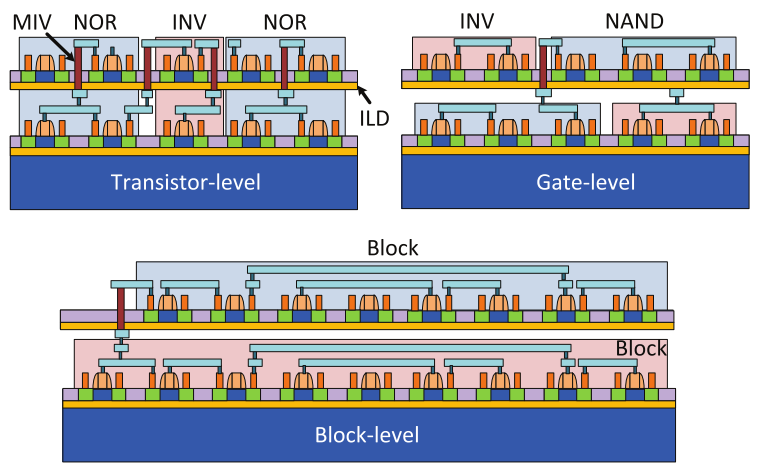
\includegraphics[width=.7\textwidth]{img/M3D-Lim.png}
	\caption{The three levels of monolithic 3D ICs: transistor-, gate- and block-level (\citet{Panth}).}
	\label{fig:m3d}
\end{figure}

The transistor-level integration can separate the transistors of standard cells on different layers of the 3D IC, enabling the finest grain integration.
However, it would require the redesign of standard cells.

The next grain level is to work on gates. %But isn't gate-level a scam? Don't they use multi-level schemes that will need to coarsen the graph (group the gates in logic blocks) before partition it? Is the uncoarsening phase really that important? Are the results so different from the block-level partitioning?
Existing standard cells can be reused, but the partitioning algorithm needs to handle millions of nodes.

Finally, monolithic 3D chips can be designed from functional blocks.
On top of being able to reuse existing standard cells, even IPs could be reused as such.
Yet, this level of integration does not take full advantage of the fine integration nature of monolithic 3D.

Monolithic has drawbacks, though.
Its sequential manufacturing is expensive and most of the wire length gained from shorter 2D connections is lost on 3D connections due to all the small nets that are cut by the partitioner.
What is worst is that the wire capacitance is even increasing due to the multiplication of nets.


\paragraph{3D stacking}
When stacking ICs to make them 3D, each layer is a full fledged IC, with its substrate and metal layers.
To bond them together, two main methods exist:
\begin{itemize}
	\item \gls{f2f}, using F2F vias (\citep{Peng2017}). We put the \gls{beol} of each chip in front of each other (see figure~\ref{fig:f2f}).
	Although this method avoids drilling through the substrate of the dies, it is limited to two layers.
	\item \gls{f2b}, using \textmu-bumps and \glspl{tsv}. The \gls{beol} of one die is stacked to the \gls{feol} of the other, this time allowing unlimited layers to be stacked (see figure~\ref{fig:f2b}).
\end{itemize}

\begin{figure}[!h]
\centering
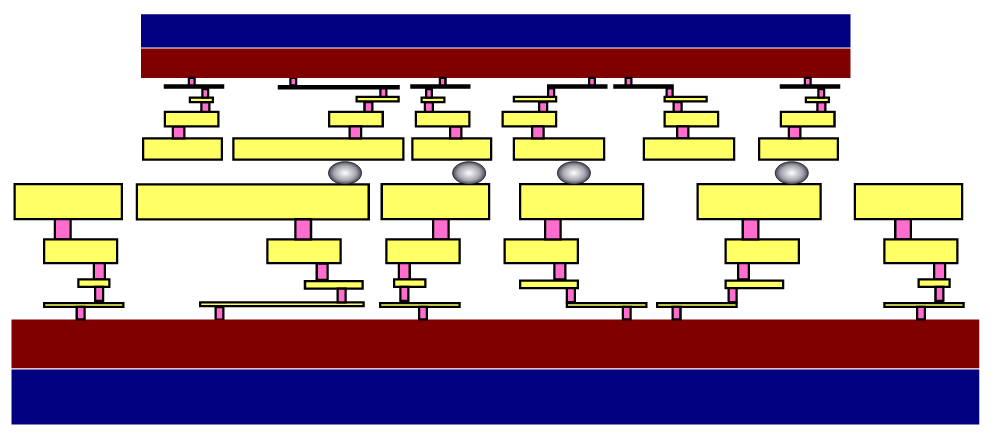
\includegraphics[width=.6\textwidth]{img/f2f.png}
\caption{Face-to-face integration, the two front-end-of-line are facing each other.}
\label{fig:f2f}
\end{figure}

\begin{figure}[!h]
\centering
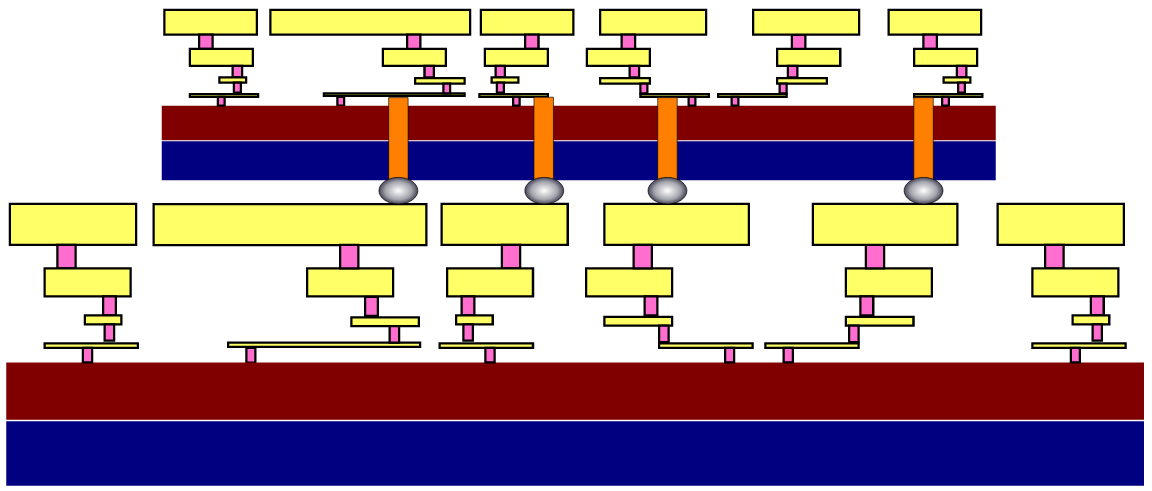
\includegraphics[width=.6\textwidth]{img/f2b.png}
\caption{Face-to-back integration, the \textmu-bumps mounted on the \gls{beol} of the bottom tier are aligned with the \gls{tsv} in the \gls{feol} of the top tier.}
\label{fig:f2b}
\end{figure}



Furthermore, there are three other methods to bond wafers together: 
\begin{itemize}
	\item \gls{w2w}, simply stack two full wafers. Easier for high-\gls{gl:yield} processes with wafers of the same size.
	\item \gls{d2w}, bond individual dies on a wafer. More complex integration, but gives a better yield (failed dies are discarded) and does not require die or wafers of the same size.
	\item \gls{d2d}, bond individual dies together. Further complicates the manufacturing process and cost due to pick-and-place operations, but the yield is further improved.
\end{itemize}


~\newline{}
The research on all families of methods is not restrained to a few research groups.
Lots of them are heavily tied with the industry and supported by public grants.
In Europe only, FP7 and H2020 project frameworks have supported or are still supporting numerous teams.\\

% TODO Remove bold and shit.
FP7 Projects:
\begin{itemize}
	\item FAB2ASM: \textit{Efficient and Precise 3D Integration of Heterogeneous Microsystems from Fabrication to Assembly}\footnote{\url{http://cordis.europa.eu/project/rcn/94309_en.html}}.
	%They aim at improving the manufacturing of 3D ICs by developing faster and more accurate techniques, such as better robotic tools and physics of self-alignment.

	\item JEMSIP\_3D: \textit{Joint Equipment and Materials for System-in-Package and 3D-Integration}\footnote{\url{http://cordis.europa.eu/project/rcn/201936_en.html}}.
	\item NANOPACK: \textit{Nano Packaging Technology for Interconnect and Heat Dissipation}\footnote{\url{http://cordis.europa.eu/project/rcn/85245_en.html}}.
	\item ELITE: \textit{Extended Large (3D) Integration TEchnology}\footnote{\url{http://cordis.europa.eu/project/rcn/85238_en.html}}.
\end{itemize}


Horizon 2020 projects:
\begin{itemize}
	\item TAKE5: \textit{Technology Advances and Key Enablers for 5 nm}\footnote{\url{http://cordis.europa.eu/project/rcn/203403_en.html}}. This projects aims at the development of the 5nm node. Even though scaling is worth exploring, the 3D integration path is not to be left aside.
	\item NeuRAM3: \textit{NEUral computing aRchitectures in Advanced Monolithic 3D-VLSI nano-technologies}\footnote{\url{http://cordis.europa.eu/project/rcn/199168_en.html}}.
	\item METRO4-3D: \textit{Metrology for future 3D-technologies}\footnote{\url{http://cordis.europa.eu/project/rcn/199865_en.html}}.
\end{itemize}
%http://cordis.europa.eu/search/result_en?q=%27Generic%27%20AND%20%27micro-%27%20AND%20%27nano-electronic%27%20AND%20%27technologies%27%20AND%20%28contenttype%3D%27project%27%20OR%20/result/relations/categories/resultCategory/code%3D%27brief%27,%27report%27%29%20AND%20programme/code%3D%27H2020*%27




\section{3D IC design flow}\label{sec:flows}
As the research in 3D IC partitioning and manufacturing advanced, it makes sense that comprehensive 3D workflows have been developed to prototype the innovations.
Here follows a selected list of some academic integration flows.

\begin{description}
	
	\item[CoolCube] In the past few years, the CEA LETI has been working on a new way to integrate transistors in 3D: \cite{Batude2015, Brunet2016, Clermidy2015, Michailos2016, Vinet2016}.
	Their goal is to manufacture 3D monolithic chips using innovative stacking techniques.
	However, they still face the problem of partitioning and gates repartition on the tiers.

	\item[Shrunk2D] Another and slightly older \gls{m3d} toolchain that shrinks the cells to evaluate the wire length and placement in 3D \citep{Panth}.
	By shrinking the dimensions by a factor $1/\sqrt2$ everything is twice as small.
	After placing and routing the shrunk cells, they are expanded back to their original size and every overlapping cells are separated on two different dies.
	This evaluation of course only works when we assume the breadth of the vertical integration to be negligible, which is a fair assumption for \gls{m3d}.

	\item[Cascade2D] An \gls{m3d} design flow developed by \citet{Chang2016} as an improvement over Shrunk2D.
	Some of its enhancements compared to its predecessor includes the addition of a \gls{miv} planning stage between the partitioning and 3D placement, the versatility of compatible partitioning algorithms and the ability to work at block-level.

	As promising as it is, Cascade2D sadly is highly interlaced with Cadence\textsuperscript{\textregistered} Innovus\textsuperscript{\texttrademark}, limiting its reusability without the proper licenses.

	\item[MEVA-3D] is a bit different from the previous tools: it is an automated design flow evaluation designed by \citet{Cong2006}.
	The team overlooks most of the 3D design to focus on the thermal dissipation and comparison between 2D and 3D architectures.
	They spend most of their effort on thermal network modeling as well as thermal via insertion in the design to ensure a correct heat flow through the layers.
	
	% \item[PathFinding] \todo{Evoqué dans 'Design Issues in Heterogeneous 3D/2.5D Integration}
	
\end{description}




%  #######   ##     ##     ###     ##         ##         #########  ##      ##   #######   #########   #######   
% ##     ##  ##     ##    ## ##    ##         ##         ##         ###     ##  ##         ##         ##     ##  
% ##         ##     ##   ##   ##   ##         ##         ##         ## ##   ##  ##         ##         ##         
% ##         #########  ##     ##  ##         ##         ######     ##  ##  ##  ##   ####  ######      #######   
% ##         ##     ##  #########  ##         ##         ##         ##   ## ##  ##     ##  ##                ##  
% ##     ##  ##     ##  ##     ##  ##         ##         ##         ##     ###  ##     ##  ##         ##     ##  
%  #######   ##     ##  ##     ##  #########  #########  #########  ##      ##  ########   #########   #######  

\chapter{Challenges: Why is it not done yet?}\label{chap:challenges}
3D is not a novel idea. In 1979, \citet{Geis1979} already demonstrated the concept.
They were followed on the 80's \citep{Akasaka1986, Colinge1981, Goeloe1981, Kawamura1983, Kunio1989, Nakano1984, Nishimura1987, Sugahara1986, Terui1983} and the 90's \citep{Neudeck1999, Saraswat1999, Strickland1998, Subramanian1998} by a lot of theoretical research on 3D CMOS and early integration.
But it is only in the 2000's \citep{Souri2000} that full workflows began to be developed and full chips manufacturing began to be considered.

The main factor why it has not been more thoroughly investigated earlier is that the cost to scale down the technology was simply lower than developing 3D integration technologies.
Hence, as attractive a research subject it was, the industry was simply not ready to heavely invest in it.

Apart from the pure manufacturing management, multiple issues arise when we tackle the 3D integration problem.
Some of those problems are exposed in this section to alert the reader to the complexity and the span of the situation.

% If I wanted to say more, I could add that those problems are the source of the complexity of the partitioning problem, obviously.
% How do you choose the metrics for your cutsize, which weights to set, when there are so many constraints to satisfy?


\section{Manufacturing}
As we already discussed in section~\ref{sec:int-flav}, there exist multiple ways to manufacture a 3D IC.
\citet{Xu2012} did a review of yield enhancement for stacked 3D IC and identified two main sources of yield loss when going 3D:
\begin{itemize}
	\item Stack yield loss.
	When stacking two dies using the \gls{w2w} technique, you may stack a bad die with a good one.
	This issue is referred to as the “known good die” problem.

	\item Assembly yield loss.
	This is simply the extension of the traditional yield loss in 2D architectures: manufacturing is a risky process and may fail.
	3D stacking further worsen the situation by adding extra steps such as wafers alignment and handling, \gls{tsv} defects and interactions with the package.
	The temperature, signal integrity and reliability of 3D ICs are affected by how the dies are stacked and where the \textmu-bumps are placed \citep{Vempati2009,Jung2012}.
	Indeed, due to the difference in coefficient of thermal expansion between the substrate and package, when the 3D IC undergo thermal load, residual stress can get transferred from the package to the substrate, degrading its reliability.
\end{itemize}

Techniques to reduce those losses respectively include pre-bond die testing and TSV redundancy to alleviate the defective ones.
However, the precise loss in yield is still unsure.
Assuming the number of defaults per unit area is constant, manufacturing smaller dies will increase the yield, but the 3D integration process may reduce the yield at the same time.
Whether both factors counterbalance is part of the challenge.



\section{Thermally-aware Design}
Manufacturing 3D IC efficiently is one thing, but having them function properly without failing is another entirely.
As the dies are stacked, the heat generated by the standard cells becomes increasingly difficult to dissipate and the reliability of the chip decreases~\citep{Lin2008}.
Farther the cells are placed from the heatsink, the more critical they get.

In the recent years, two research directions have emerged to address this problem:
\begin{itemize}
	\item Thermal co-design~\citep{Cong2004, Cong2007, Minz2008, Ryu2011, Zhang2006}: either by cleverly spreading the cells on the dies to limit the hotspots and heat gradient, or by using thermal \gls{tsv}s whose role is to canalize and improve the heat flow through the layers.
	For example, by forcing the high-power cells on the layer closer to the heat sink, \citet{Athikulwongse2014} outperforms state-of-the-art temperature aware placers by 10\% and 33\% in terms of maximum temperature and temperature difference.
	
	\item Micro-fluidic cooling~\citep{Koo2005, Serafy2013, Serafy2016}: leave space between the layers and use some deionized fluid to evacuate the heat channeled through inter-tiears fins.
	Advocates of this technique argue that micro-fluidic cooling improves performance and efficiency of a given architecture compared to traditional air cooling.
	If it seems promising on paper, it is a complex technology to put into practice, as it further complicates the manufacturing and needs a paradigm shift of chips integration in complete systems.
\end{itemize}


% \subsection{Find appropriate metrics}
% \todo[inline]{Extract the most common from the Sung Kyu Lim's papers}
% \begin{itemize}
% 	\item Area reduction (\citep{Chan2017})
% 	\item Power reduction (\citep{Chan2017})
% 	\item WL reduction (\citep{Chan2017})
% 	\item Longest path delay (\citep{Athikulwongse2014})
% 	\item gate and wire capacitance \citep{Chang2016}
% \end{itemize}

\section{Clock Tree Synthesis}
When synthesizing a clock tree, we want to avoid clock skew (maximum difference in clock arrival between sinks)~\citep{Lu2017}.
% Already a challenge in 2D, the matter is worse in 3D, espacially for the fabrication.
We could have separate clock I/Os on each layer to enable single-die clock testing and increasing the yield.
Indeed, current \gls{cts} need the full bonded chip to be tested.
If die \gls{cts} could be tested individually, even more failed dies could be discarded early in the manufacturing process.


\section{Power Delivery Network}
The \gls{pdn} also needs to be revised when going 3D.
When the power needs of the IC scale with the area footprint and number of layers, the pins needed to deliver this power from an external source are still limited by the same footprint of the chip.
The imbalance is a challenge \citep{Jain2008}.

What can be even more of a challenge is when we consider an air-cooled 3D IC.
The power delivery pins and heatsink are on opposite sides of the chip, but the same type of cells need them the most at the same time.
The most power consuming cells should be placed close to the power source in order to avoid a complex \gls{pdn}, but at the same time they will dissipate the most heat and should be placed to the heatsink to avoid failures.
Teams working on the problem are trying to optimize the power demand across layers, such as \citet{Pantht2015} who developed a \gls{pdn} aware gate-level  partitioner.



% ##           ##    #####    ########   ##   ##    
% ##           ##  ##     ##  ##     ##  ##  ##     
% ##           ##  ##     ##  ##     ##  ## ##      
% ##           ##  ##     ##  ########   ####       
%  ##   ###   ##   ##     ##  ##   ##    ##  ##     
%   ## ## ## ##    ##     ##  ##    ##   ##   ##    
%    ###   ###       #####    ##     ##  ##    ##  

\chapter{Work: Where are we now?}\label{sec:work}\label{chap:work}
Nowadays, there is still not any commercial 3D IC design toolchain.
Our aim is to bring an interface between existing 2D tools to enable automatic 3D integration, and reducing as much as possible the proprietary intermediaries, in order to keep the flow as open as possible.
As we discussed in section~\ref{sec:flows}, some academic toolchains are already pushed by different research teams around the globe.
Their common divisor is their ties to specific, expensive tools and their lack of flexibility.
This is a major drawback we want to alleviate in our work.

The figure~\ref{fig:flow} gives a macroscopic idea of the interface we aim at developing.
The elements on the left-hand side are existing solution and tools, while the right-hand blocs are currently developed to automate what is currently mainly done by hand.

\begin{figure}[!h]
	\centering
	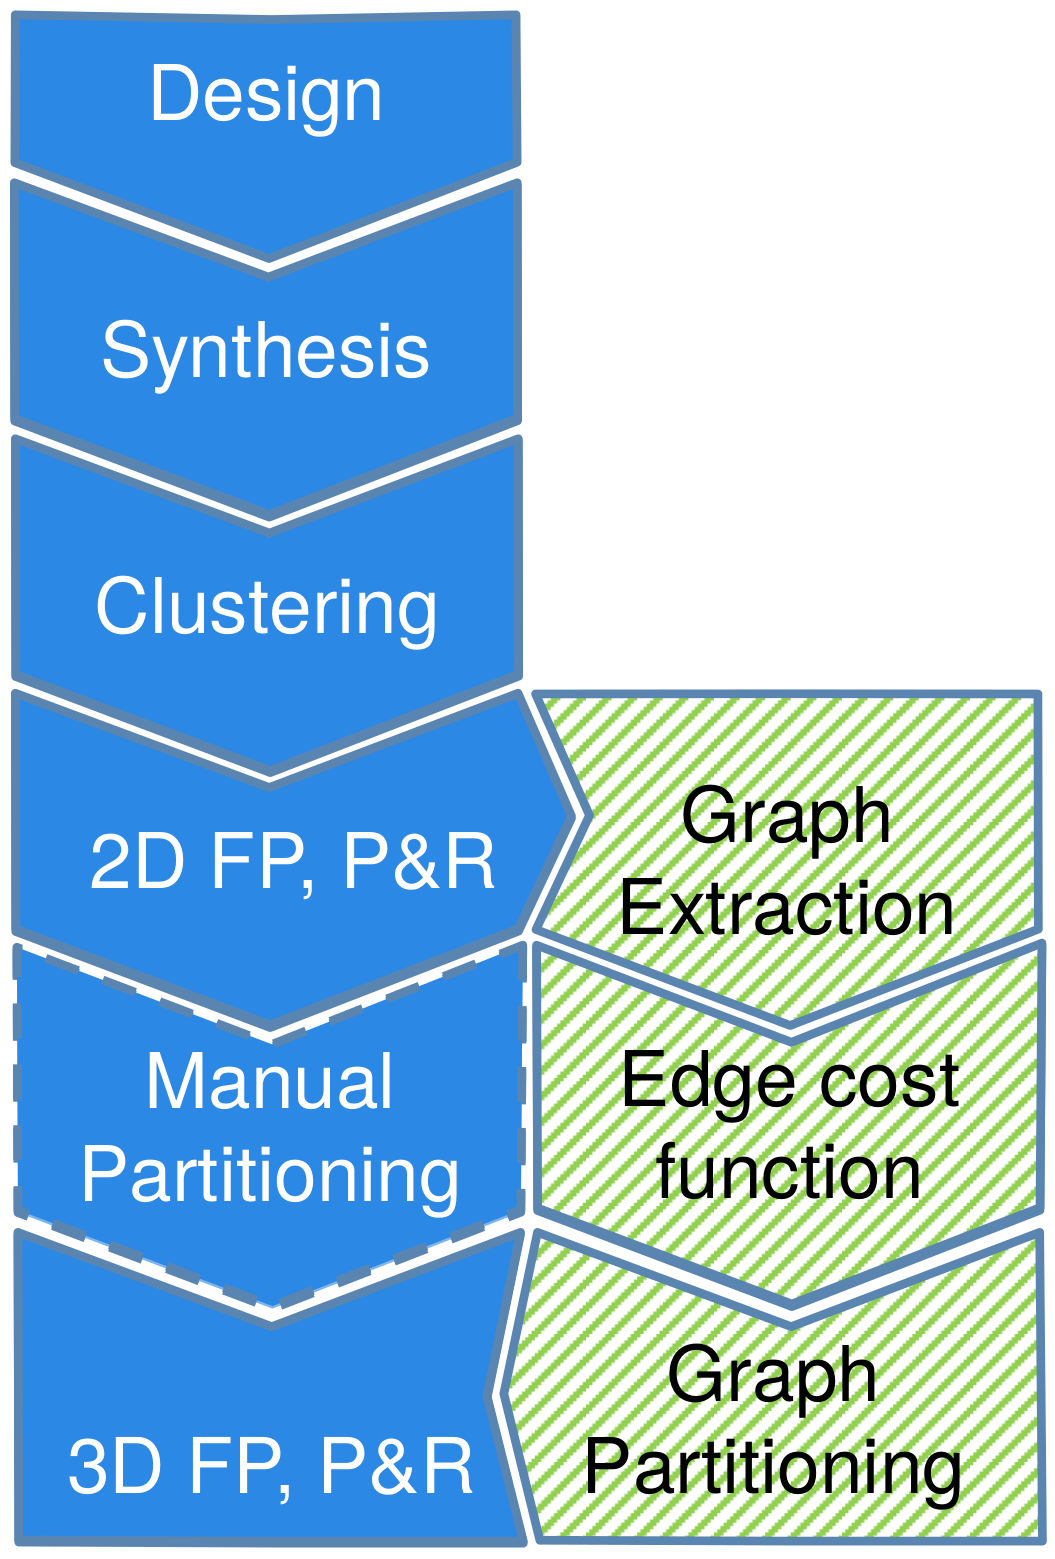
\includegraphics[width=.35\textwidth]{img/flow.png}
	\caption{Typical 3D IC design flow. We want to bypass the usual manual partitioning with an automated graph extraction and partitioning.}
	\label{fig:flow}
\end{figure}

In this section, we will present what has been developed so far and how those components interact with each other.

% \todo[inline]{Quelles sont mes contributions ? Je ne peux pas simplement leur dire que j'ai développé deux scripts qui utilisent le travail d'autres personnes, c'est ridicule. Mes contributions doivent provenir de l'analyse des résultats et leur obtention. Par exemple pour def\_parser : je me suis affranchi de l'extraction de statistiques classique utilisée dans les outils commerciaux. En partant du fichier .def standard, on peut obtenir les mêmes informations. Ces informations sont extrêmement utiles dans le sens où elles permettent de mettre en évidence le lien entre le grain du clustering et l'interconnectivité des clusters, et ce peu importe l'architecture. Il y a clairement une corrélation qui nous permettrait de dire que les résultats obtenus pour une architecture typique sont transposables dans une certaine mesure à d'autres architectures similaires. En ce qui concerne PHONEY, c'est un framework complet qui permet de facilement comparer différentes implémentations d'algos de partitionnement en utilisant des métriques personnalisées. C'est un moyen de tester et fine-tuner les algos à utiliser partitionner les architectures. Ces deux outils sont aussi interfaçables entre eux afin d'assurer la continuité du workflow. Parmi les étapes suivantes, on peut évoquer la comparaison de PaToH et hMetis et pourquoi pas d'autres implémentations, la génération de netlists partitionnées, etc.}

\section{Graph Extraction}\label{sec:graph-extr}
We developed \texttt{PHONEY}\footnote{“Partitioning of Hypergraph Obviously Not EasY”, \url{https://github.com/parastuffs/metis_unicorn/blob/master/script/phoney.py}}, a software tool extracting the hypergraph of a 2D placed and routed design, feeding it to a partitioner and formating the output for the \gls{pr} tool to process back.
The processing is pretty straightforward: each cluster of the design becomes a vertex and whenever a net is connecting cells belonging to different clusters, the net becomes an hyperedge.
The (hyper)graph is then formated in such a way that the partitioner can do its job and generate nice and clean partitions.
The partitioner in question can be any library with a command-line interface; all that is needed is one function translating our representation of a graph into one understandable by the library.
So far, we support METIS, hMETIS and PaToH.
The support for METIS was added to compare the partition quality between a hypergraph and its corresponding graph.
Notwithstanding the motivation for hypergraphs we discussed in section~\ref{sec:why-hypergraph}, we did not note a significant difference in quality between the two approaches.


~\newline{}
Here follows a summary of the main features of \texttt{METIS}:
\begin{itemize}
	\item Extract the design as a graph or hypergraph.
	\item Choice of the partitioner: METIS, hMETIS or PaToH.
	\item Disbalance of the graph weights power-wise. This can either be done by inserting a dummy node or by manually overriding the partitioning and moving nodes around “by hand”. Those are further discussed in section~\ref{sec:asym-part}.
	\item Type of edge weights.
	\item The script and partitioner can be seeded, insuring repeatability of the results.
\end{itemize}


% We use the outputs from Cadence(?) P\&R to extract the vertices and hyperedges, as well as the weights of the graph.

\section{Stats extraction and interface with open standards}
The extraction of statistics about the design is essential to the weights of the graph.
Those can either be obtained through the analysis of a third-party software or from the output of the \gls{pr} tool.

In the early days of our flow, \texttt{PHONEY} was only able to read a proprietary tool-specific file formatting.
Although the format was documented and consisted of standard text files, you needed to be aware of it if you wanted to use the script.
With the addition of \texttt{def\_parser}\footnote{\url{https://github.com/parastuffs/def_parser}}, our toolchain is now compliant with the open standards \gls{def} and \gls{lef}.
This script feeds on a \gls{def} file containing all the information on the placed and routed design, and on an associated \gls{lef} file containing the physical description of the standard cells of the specific technology used.

One of its role is to translate those standard files into an input that \texttt{PHONEY} is able to process.
The other is to cluster and analyze the design.

~\newline{}
Here follows a summary of the main features of \texttt{def\_parser}:
\begin{itemize}
	\item Compatibility with open standards.
	\item Extract all the cells, pins and nets of the design and their interconnection.
	\item Analyze the geometry of the die.
	\item Design clustering (see section~\ref{sec:clustering} and analysis).
\end{itemize}


\section{Naive Clustering}\label{sec:clustering}

The aim of our clustering is manyfold: (i) reduce the order of the graph for the partitioner to have an easier job, (ii) slice the die and analyze the interconnectivity between the clusters, (iii) be a proof-of-concept clustering that allows us to already prepare the extraction of statistics for more complex clustering methods that may replace this one.

The way it is implemented is simplistic and naive: we slice the die into a grid with each cell being a cluster.
We consider that the \gls{pr} has placed close to each other standard cells that participate to the same logical function, hence making them a sound logical block that can be used as a cluster.
By playing on the granularity of the clustering, we hope to highlight the impact of inter-cluster wire length when tackling the gate- or block-level dilemma.

As we will see in chapter~\ref{chap:results}, this geometrical clustering also allows us to proceed to a first, rough study of the interconnection of standard cells in a given design.







% ########   #########   #######   ##     ##  ##         ##########   #######   
% ##     ##  ##         ##     ##  ##     ##  ##             ##      ##     ##  
% ##     ##  ##         ##         ##     ##  ##             ##      ##         
% ########   ######      #######   ##     ##  ##             ##       #######   
% ##   ##    ##                ##  ##     ##  ##             ##             ##  
% ##    ##   ##         ##     ##  ##     ##  ##             ##      ##     ##  
% ##     ##  #########   #######    #######   #########      ##       #######  

\chapter{Results: What can we say?}\label{chap:results}
In this chapter, we will analyze the results of some partitioning using \texttt{PHONEY} and hMETIS as well as some clustering computed by \texttt{def\_parser}.
We focus on \gls{wl} reduction (section~\ref{sec:wl}), power asymmetry (section~\ref{sec:asym-part}), and inter- and intra-clustering connectivity (sections~\ref{sec:res-intercl} and \ref{sec:res-intracl}).






\section{Wire length reduction}\label{sec:wl}

For the sections \ref{sec:wl} and \ref{sec:asym-part}, we used three different sub-modules of the OpenSPARC T2, each with different level of wire or gate dominance (see table~\ref{tab:arch}).

\begin{table}[!h]
	\centering
	\begin{tabular}{ccc}\hline
	SPC (Core) & CCX (Crossbar) & RTX (Ethernet) \\ \hline
	Gate dominated & Wire dominated & Balanced \\
	\end{tabular}
	\caption{The three modules tested with our partitioning flow, each with a different level of gate or wire dominance.}
	\label{tab:arch}
\end{table}

Using \texttt{PHONEY}, we extracted the following weights for our graphs:
\begin{itemize}
	\item Edges:
	\begin{itemize}
		\item Number of wires per connection
		\item Total wire length of the hyperedge
		\item Average wire length of the nets in the hyperedge
		\item Linear combination and inverse of those
	\end{itemize}
	\item Vertices:
	\begin{itemize}
		\item Area
		\item Power
	\end{itemize}
\end{itemize}

Note that if the partitioner supports multiple weights at the same time for the vertices, the edges can only be characterized with a single weight.

Our first objective was to find out the potential of our workflow by studying the \gls{wl} reduction when going 3D.
The figure~\ref{fig:res-3dwl} summarizes two reductions: the total \gls{wl} and the longest net shortening.

\begin{figure}[!h]
\centering
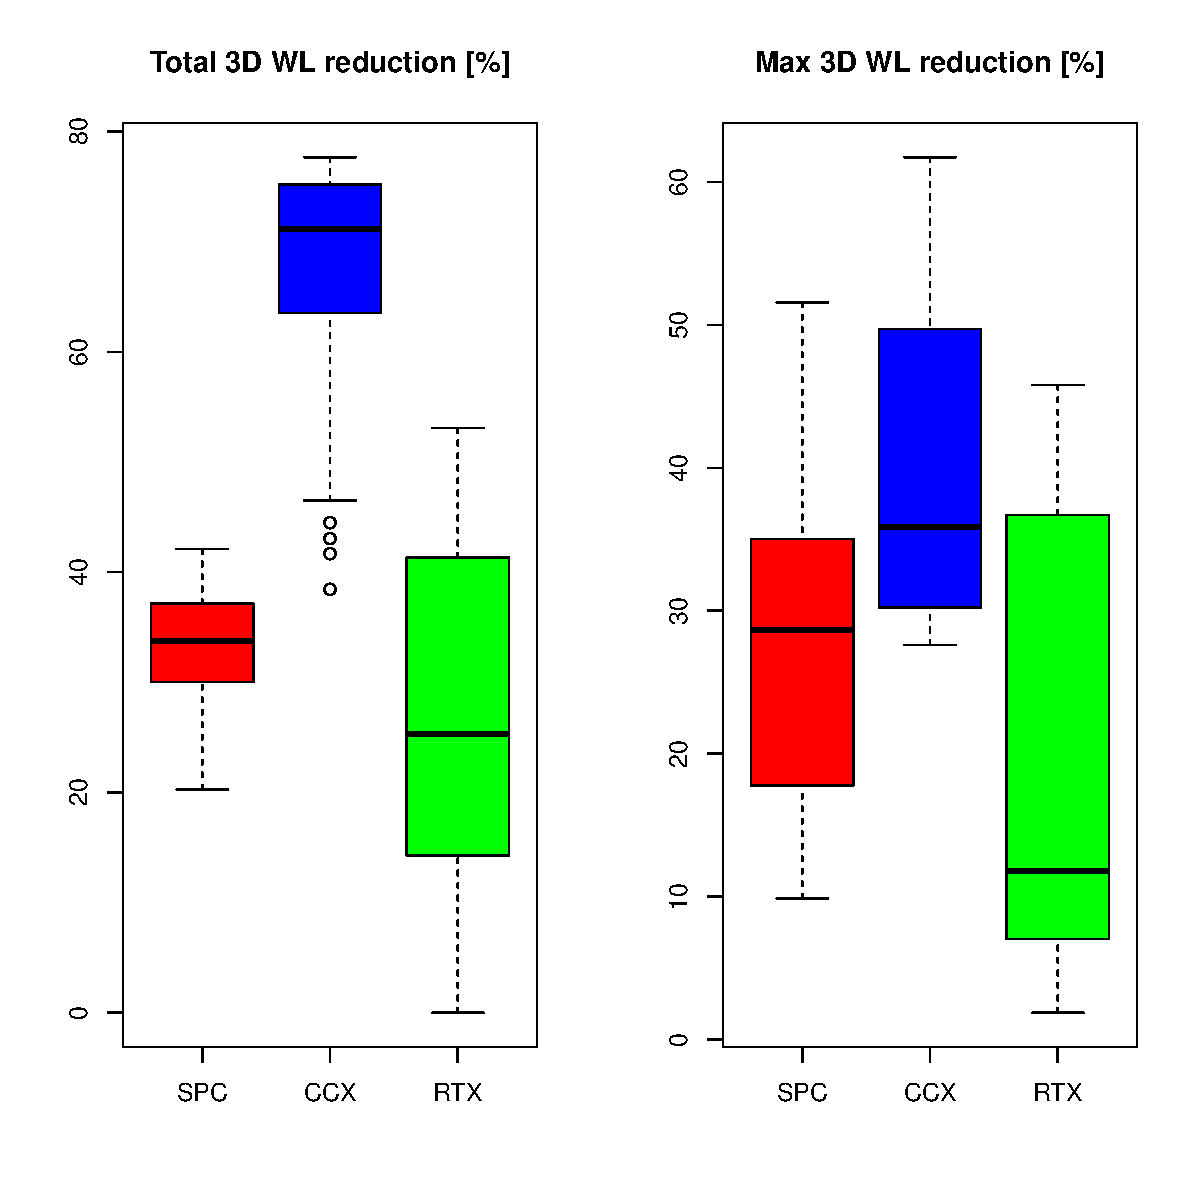
\includegraphics[width=.8\textwidth]{img/3DWL.pdf}
\caption{Total and maximum wire length reduction when going 3D.}
\label{fig:res-3dwl}
\end{figure}

We could have expected RTX to yield results between SPC and CCX due to its balanced design.
However, whilst there are some gains, the median is worse than SPC.
% This can be explained by the pre-clustering of the architecure that is probably too coarse for such a small module.
A more interesting result about RTX is that its set of solutions spans from $0$ to $53\%$ \gls{wl} total reduction, showing that for some designs, the choice of appropriate metrics is critical.
At the same time, the difference between the first and third quartile of SPC is only around $7\%$.
Contrarily to RTX, other designs do not depend heavily on the metric, but this seems to be more of a corner case.

All in all, the quality of the partitioning depends on the weights used on the hypergraph and should not be picked lightly.
Following our experiments, wire-dominated designs such as CCX can hope for up to $77\%$ (median $71\%$) of wire length reduction and $61\%$ (median $35\%$) of longest net reduction.




\section{Asymmetric partitions}\label{sec:asym-part}
One of the limitations of popular implementations is their mania with balanced partitioning.
For example, hMetis allows the user to set loose balance constraints, but will still try to produce partitions as balanced as possible.
If we want to produce asymmetric (\textit{i.e.} unbalanced) partitions, we need to trick the partitioner.

Say we want an asymmetric repartition of power on two dies of the same size.
This gives two balance objectives the partitioner needs to follow.
To unbalance only one of them, we can create a fake, dummy node with a fixed power density and a negligible area.
Doing so, the partitioner will still balance both metrics, but the actual power balance will be offset.
For example, a $70/30$ imbalance can be achieved by creating a dummy node with a power equal to $40\%$ of the total power.
The partitioner is then fooled into thinking it needs to balance $140\%$ of this metric, from which the dummy node will ultimately be removed.

By using the fixed vertices feature that most libraries implement, we can then choose the repartition of the asymmetry.\\

In practice, we tested this idea on the SPC module and obtained the results on figure~\ref{fig:res-asym}.

\begin{figure}[!h]
\centering
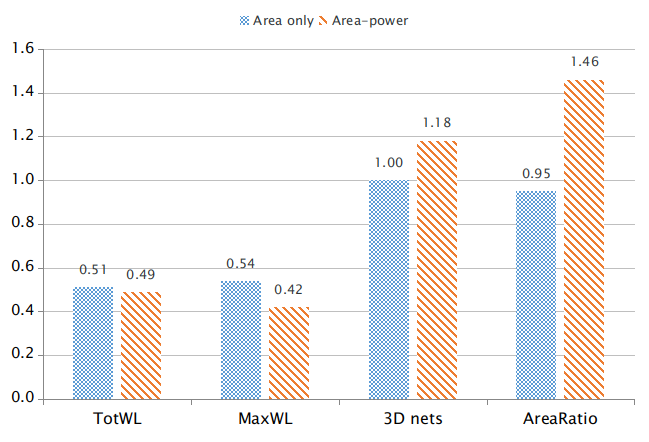
\includegraphics[width=.8\textwidth]{img/res-asym-power}
\caption{By forcing the asymmetry power-wise, we further gain some total wire length shorten the longest net, but there are globally more 3D nets and the aspect ratio is unbalanced. All values are the ratio between the 3D and 2D implementation.}
\label{fig:res-asym}
\end{figure}

In the end, although the $70/30$ power disbalanced objective is reached, the area balanced could not be maintained and drops to $60/40$.
By using a less aggressive asymmetry objective, we were able to conserve the area balance, but with close to no gain to the wire length.
%Note: I don't even know which die hoted the higher power. I suppose the largest of the two.
Still, even though the two dies do not have the same size anymore, the disbalance allowed us to further reduce the total wire length by 2\% and the maximum wire length by 12\%, to the cost of an extra 18\% of 3D nets.








\section{Inter-cluster connectivity}\label{sec:res-intercl}
%Ces informations sont extrêmement utiles dans le sens où elles permettent de mettre en évidence le lien entre le grain du clustering et l'interconnectivité des clusters, et ce peu importe l'architecture. Il y a clairement une corrélation qui nous permettrait de dire que les résultats obtenus pour une architecture typique sont transposables dans une certaine mesure à d'autres architectures similaires.
To test our clustering and analyze it, we used some new designs at two different technology nodes (see table~\ref{tab:arch-clust}).

% TODO find a way to align the numbers.
\begin{table}[!h]
\centering
	\begin{tabular}{l|c|c|c|c}
	Design@tech & Cells & Nets & Total \gls{wl} [$\mu m$] & Area [$\mu m^2$] \\ \hline
	SmallBoom@7nm & $121\,580$ & $137\,171$ & $308\,947$ & $10\,401$ \\
	% RTX &&&& \\
	Flipr@7nm & $220\,587$ & $234\,373$ & $767\,365$ & $14\,713$ \\
	LDPC@7nm & $42\,471$ & $49\,633$ & $173\,167$ & $3\,309$ \\
	SPC@45nm & $289\,812$ & $306\,118$ & $10\,112\,735$ & $906\,827$ \\
	CCX@45nm & $185\,777$ & $200\,999$ & $5\,455\,493$ & $313\,464$ \\
	\end{tabular}
\caption{List of all tested architectures: Either using 45nm or 7nm standard cells library.}
\label{tab:arch-clust}
\end{table}

The aim of this experiment is to highlight similarities between the designs and try to find tendencies of the impact of clustering on interconnection and wire length.
The results are summarized on figures~\ref{fig:res-intercl-totnet-7nm}, \ref{fig:res-intercl-totnet-45nm}, \ref{fig:res-intercl-totwl-7nm} and \ref{fig:res-intercl-totWL-45nm}.

% \begin{figure}
% \centering
% 	\begin{subfigure}[b]{.45\textwidth}
% 		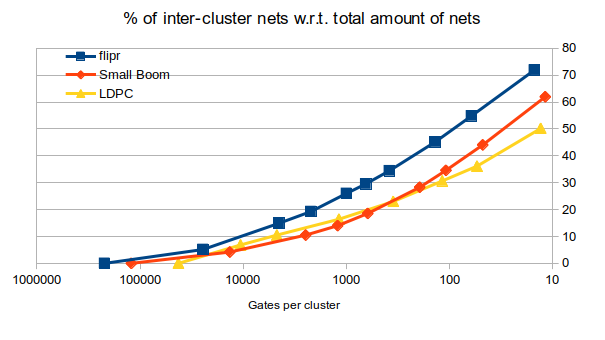
\includegraphics[width=\textwidth]{img/res-inter-cluster-totalnets-7nm.png}
% 	\end{subfigure}
% 	\begin{subfigure}[b]{.45\textwidth}
% 		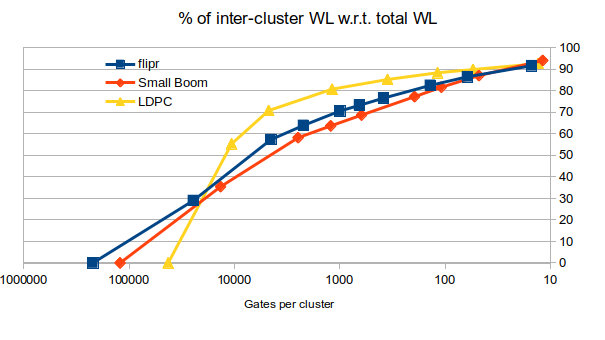
\includegraphics[width=\textwidth]{img/res-inter-cluster-totalWL-7nm.png}
% 	\end{subfigure}
% 	\begin{subfigure}[b]{.45\textwidth}
% 		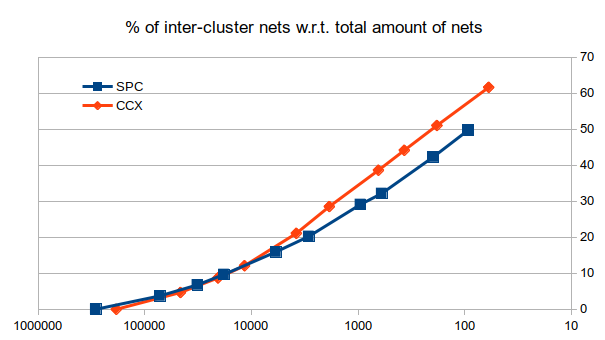
\includegraphics[width=\textwidth]{img/res-inter-cluster-totalnets-45nm.png}
% 	\end{subfigure}
% 	\begin{subfigure}[b]{.45\textwidth}
% 		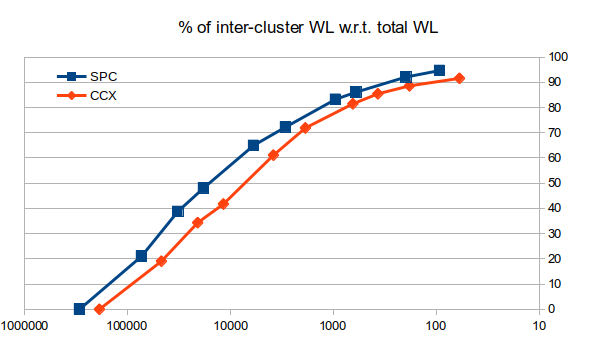
\includegraphics[width=\textwidth]{img/res-inter-cluster-totalWL-45nm.png}
% 	\end{subfigure}
% 	\caption{Lots of graphs.}
% 	\label{fig:res-inter-cluster}
% \end{figure}
\begin{figure}[!h]
	\centering
	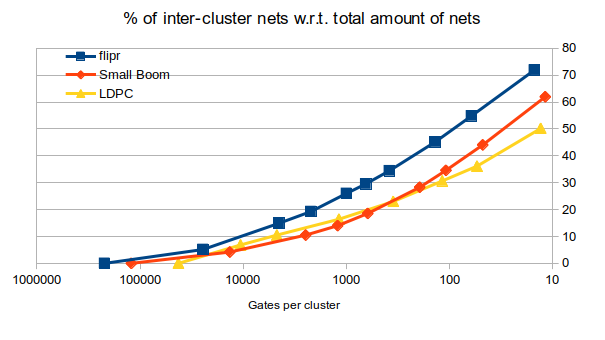
\includegraphics[width=.9\textwidth]{img/res-inter-cluster-totalnets-7nm.png}
	\caption{Percentage of inter-cluster nets \textit{w.r.t.} the total amount of nets for the 7nm designs.}
	\label{fig:res-intercl-totnet-7nm}
\end{figure}
\begin{figure}[!h]
	\centering
	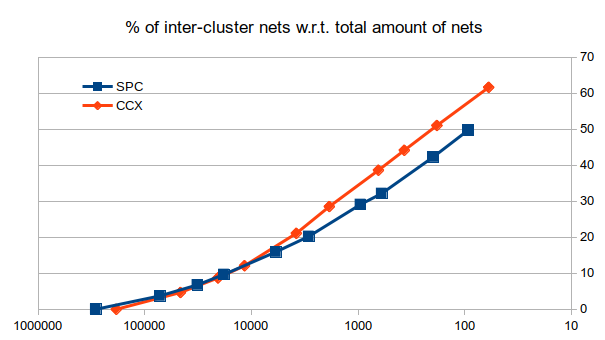
\includegraphics[width=.9\textwidth]{img/res-inter-cluster-totalnets-45nm.png}
	\caption{Percentage of inter-cluster nets \textit{w.r.t.} the total amount of nets for the 45nm designs.}
	\label{fig:res-intercl-totnet-45nm}
\end{figure}

~\newline{}
First, the figures~\ref{fig:res-intercl-totnet-7nm} and \ref{fig:res-intercl-totnet-45nm} show the number of nets that span over several clusters.
As it was expected, the proportion increases the finner the clustering gets.
All five designs follow the same trend with some disparities when the clusters become really small, which is not surprising either.
With very small clusters, the particularities of each design tend to take over the general trend.

From those results, we can say that the finner the grain, the more nets will need to be considered in the partitioning, but we have some margin.
Indeed, most automatic clustering tools (either hierarchical, logical or geometrical) limit themselves from a few dozens up to a hundred-ish clusters.
Based on table~\ref{tab:arch-clust}, for 100 nodes, we are well under $30\%$ of total nets that will play a role in the partitioning.



\begin{figure}[!h]
	\centering
	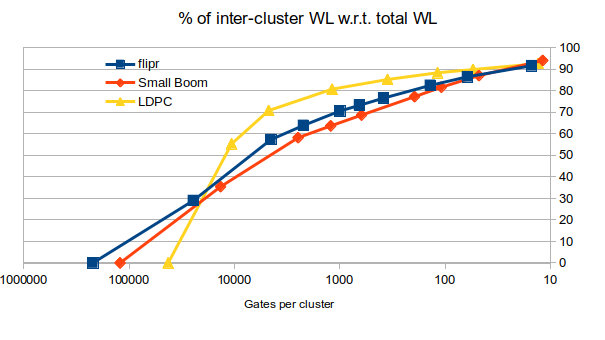
\includegraphics[width=.9\textwidth]{img/res-inter-cluster-totalWL-7nm.png}
	\caption{Percentage of inter-cluster \gls{wl} \textit{w.r.t.} the total \gls{wl} for the 7nm designs.}
	\label{fig:res-intercl-totwl-7nm}
\end{figure}
\begin{figure}[!h]
	\centering
	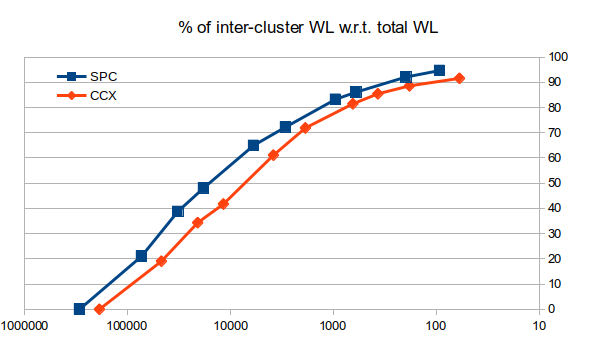
\includegraphics[width=.9\textwidth]{img/res-inter-cluster-totalWL-45nm.png}
	\caption{Percentage of inter-cluster \gls{wl} \textit{w.r.t.} the total \gls{wl} for the 45nm designs.}
	\label{fig:res-intercl-totWL-45nm}
\end{figure}

~\newline{}
Second, the figures~\ref{fig:res-intercl-totwl-7nm} and \ref{fig:res-intercl-totWL-45nm} again show the same tendencies for both technology nodes and all designs (with LDPC deviating a little).
If we consider the same situation as before, that is 100 nodes, between 60\% and 80\% of the total wire length is spanning several clusters and may be cut during the partitioning.

The objective of the clustering is to have as little nets to cut as possible, while still playing with as much wire length as possible.
To find the sweet spot, both metrics need to be analyzed at the same time.
When comparing the pairs of graphs for each technology node, a clustering embedding between 1000 and 5000 gates seems to be a nice match.








\clearpage
\section{Intra-cluster connectivity}\label{sec:res-intracl}
The intra-cluster connectivity counts the number of nets that are entirely contained inside a single cluster.
This metric helps identifying the different zones of the architecture: highly or loosely connected.

For our intra-cluster study, we will focus on the LDPC architecture, as the other designs gave similar results.

\begin{figure}[!h]
\centering
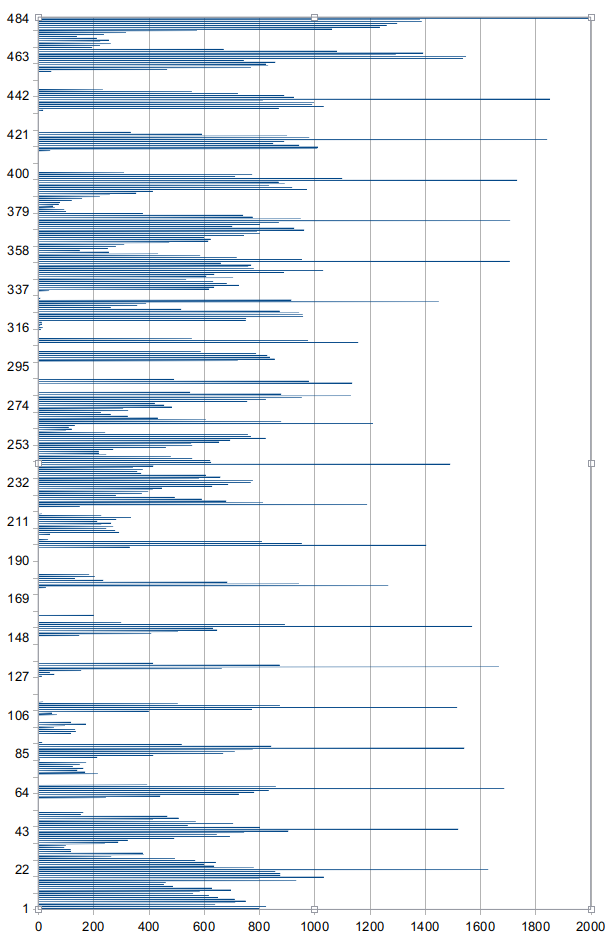
\includegraphics[width=.8\textwidth]{img/intra-clust-con}
\caption{Intra-cluster connectivity for the LDPC architecture. The clustering applied is geometrical and each cluster is numbered from 1 in the lower left corner of the die to 484 in the top right corner and progressing on horizontal rows of 22 clusters.}
\label{fig:intra-clust-con}
\end{figure}
% 484 clusters for LDPC@7nm => roughly 88 cells per cluster

A pattern emerges from the figure~\ref{fig:intra-clust-con}.
We can see that the clusters on the edge of the die have a lot of intra-connections.
This can be explained by the pins and I/O being on the border as well.
More interestingly, it shows us that a lot of clusters do not have any exclusively-intra nets.
When our partitioning objective is to reduce the 3D nets, we should not increase the number of clusters at the borders as it would increase the inter-cluster connectivity and potentially the amount of 3D nets.
On the other hand, the clusters without intra-nets could be even more reduced without creating new intercluster nets.

This metric could be used to move our clustering from naive to a bit more clever: by identifying the parts with higher intra-connectivity density, we could implement an adaptative grain coarsening, coarser at the border and finner in the inside.



% #########  ##     ##  ##########  ##     ##  ########   #########  
% ##         ##     ##      ##      ##     ##  ##     ##  ##         
% ##         ##     ##      ##      ##     ##  ##     ##  ##         
% ######     ##     ##      ##      ##     ##  ########   ######     
% ##         ##     ##      ##      ##     ##  ##   ##    ##         
% ##         ##     ##      ##      ##     ##  ##    ##   ##         
% ##          #######       ##       #######   ##     ##  #########  

\chapter{Future}\label{chap:future}
% \todo[inline]{Il me reste à défénir des questions de recherche. Quel est mon but ? Qu'est-ce que je cherche ?%
% L'un des problèmes qu'on explore, c'est la comparaison entre le monolithique et le 3D stacking. Lequel est le meilleur ? Vers quelle technologie se tourner pour fabriquer des puces en 3D fiables et rentables ? Pour le moment, on penche vers le 3D stacking en argant que le monolithique demande une intégration trop fine qui mènerait vers une énorme overhead en terme d'interconnectivité et de routing. De plus, le monolithique est plus compliqué à frabriquer et c'est justement pour faciliter la fabrication de puces à plus haute densité qu'on essaie de passer en 3D. On n'essaie pas de remplacer une 2D compliquée à frabriquer et scaler en une 3D encore plus compliquée et risquée.}
% \section{Research questions}
Many questions motivate this work and many more arise.
However, we need to focus on a subset of the problem pool.

First, the comparison between monolithic and stacking: which is the best choice?
Toward which technology turn if we want efficient and profitable 3D ICs?
We hope that our research into clustering grain and interconnectivity will help this problem moving forward.

Second, the lack of open source 3D toolchain.
By developing each link in our chain as openly and flexible as possible, we try to work toward this objective.

Third, the limitation of layers.
When talking about 3D integration today, we are still limited to two dies.
In the future, we hope to lift this limitation and open the automated 3D integration to $n$ layers.

~\newline{}
This final chapter present some of the future directions our work will take.



\section{Verilog partitioning}
When partitioning an architecture, the output is a directive file telling the \gls{pr} tool on which die to place each cluster or standard cell.
The tool then generates the appropriate signals for the dies to communicate together and a gate-level netlist for each die that will then be floorplanned, placed and routed as usual.

The next step in the tool independence is to develop the netlist generation ourselves.
Doing so will require each cut net to be converted into an external signal on both ends of the cut and connecting it correctly in the netlist.



\section{Accessibility/UI}
Although the toolchain is currently working, it is quite cumbersome to use.
All the configuration is set through a bunch of global variables and the lack of documentation is not helping.

In order for the toolchain to gain in quality, a proper user interface needs to be developed and some documentation to be written.




\section{Clustering}
As presented in section~\ref{sec:mul-para}, the multilevel paradigm already clusters the vertices of the graph during the coarsening phase.
The purpose of the naive clustering we are applying on the design, is (i) to reduce the order of the graph before feeding it to the partitioner, and (ii) maintain the integrity of logical blocks, hence easing the subsequent \gls{pr} of the partitioned dies.
At the moment, we do not yet need a very efficient clustering for the current purpose.
A future improvement could be to develop a more sophisticated algorithm that could replace the coarsening and uncoarsening of the multilevel paradigm, allowing us to fall back on a raw graph partitioning algorithm.

This would also be the occasion to test the validity of the discussion between gate- and block-level partitioning.
With the rise of multilevel schemes, a gate-level graph would need to be coarsened before the actual partitioning can take place.
That clustering would group the gates into pseudo-logical blocks (depending on the coarsening algorithm used) that could be close to the block-level graph.
In that case, is there even a sense in differentiating the two approaches?
% Hasn't this been done before? Probably.
% When Sung Kyu Lim presents the advantes of gate-level integration, does he compare the partitionings against a block-level study? I'm not sure, he's never really clear on his methods.

Furthermore, as discussed in section~\ref{sec:res-intercl}, the stake of clustering is finding the sweet spot between a low number of nets cut, and a high amount of wire length to play with and decrease.
A way to achieve this may be to exploit the results of section~\ref{sec:res-intracl} and develop an adaptative clustering method that would preserve the integrity of block with short length connections.




\section{New metrics}
Now that we are able to analyze the connectivity of clusters, it would be interesting to implement those analysis into the partitioner through a new set of weights.
Here follows some weights worth investigating:
\begin{itemize}
	\item The ratio of nets inside a hyperedge \textit{w.r.t.} the total amount of nets.
	\item The ratio of inter- over intra-cluster nets.
	\item A linear ranking based on the wire length, with the highest weight granted to the longest net.
\end{itemize}



\section{Multi-die partitioning}
If two-way partitioning is pretty straightforward, stacking three or more dies becomes more difficult.
How do we ensure the N+1 die can be connected with the N-1?
How do we penalize the connection between distant layers in the hypergraph representation?
Those are some questions that need answers if we want to enable multi-die integration in our workflow.

\section{Extended support for partitioners}
We intend to extend the suport of \texttt{PHONEY} to new partitioning libraries and improve their configurability through the script.

\clearpage

\newpage
% \nocite{*}
\bibliographystyle{abbrvnat}
% \bibliographystyle{acm}
\bibliography{../thesis/bibliography.bib}

\end{document}
